\documentclass[12pt, a4paper]{article}

\newcommand{\kafedra}{ИИТ} % Кафедра X

\newcommand{\numberOfLab}{11/12} % Лабораторная работа №X
\newcommand{\semestr}{2} % За X семестр
\newcommand{\distiplina}{ОАиП} % По дисциплине <<X>>
\newcommand{\labTitle}{Структуры, перечисления, объединения. / Бинарные и текстовые файлы} % Тема: <<X>>

% Выполнил
\newcommand{\kurs}{1} % Студент X курса
\newcommand{\group}{ПО-4 (1)} % группы X
\newcommand{\labAuthor}{Галанин П. И.} % X

% Проверил
\newcommand{\teacherStatus}{ст. преподаватель} % X
\newcommand{\teacher}{Хацкевич М. В.} % X

\newcommand{\labDate}{Брест, 2020} % X

\usepackage{../../../sty/encoding} % кодировка
\usepackage{../../../sty/titlePage} % титульный лист
\usepackage{../../../sty/fields} % поля
\usepackage{../../../sty/imgs} % картинки
\usepackage{../../../sty/code} % исходный код
\usepackage{../../../sty/labData} % для лабораторной

\begin{document}

% = = = = = Титульный лист
\maketitle
\setcounter{page}{2}

% = = = = = Содержание
\renewcommand{\contentsname}{Содержание}
\tableofcontents
\newpage

% = = = = = Тема ЛР
\labheading

% = = = = = Цель
\labgoal{
\begin{enumerate}
    \item Изучить синтаксис и правила работы со структурами. Реализовать программу с применением структур, перечислений и объединений.
    \item Изучить принципы программирования с использованием бинарных файлов. Ознакомиться с основными функциями в Си для работы с бинарными файлами.
\end{enumerate}
}

% = = = = = Ход Работы
\labreport

% = = = = = Структура проекта
\section{Структура проекта}
        \begin{verbatim}
.
├── Makefile
└── src
    ├── lab
    │   ├── lab.c     
    │   ├── lab.drawio
    │   ├── lab.h     
    │   ├── lab.png   
    │   ├── lab.tex   
    │   └── menu
    │       ├── del_data
    │       │   ├── del_data.c     
    │       │   ├── del_data.drawio
    │       │   ├── del_data.h     
    │       │   ├── del_data.png
    │       │   └── del_data.tex
    │       ├── input_data
    │       │   ├── input_data.c
    │       │   ├── input_data.drawio
    │       │   ├── input_data.h
    │       │   ├── input_data.png
    │       │   └── input_data.tex
    │       ├── menu.c
    │       ├── menu.drawio
    │       ├── menu.h
    │       ├── menu.png
    │       ├── menu.tex
    │       ├── out_data
    │       │   ├── out_data.c
    │       │   ├── out_data.h
    │       │   ├── out_data.png
    │       │   └── out_data.tex
    │       └── sort_data
    │           ├── sort_data-get_sorted_array.png
    │           ├── sort_data-sort_data.png
    │           ├── sort_data.c
    │           ├── sort_data.drawio
    │           ├── sort_data.h
    │           ├── sort_data.tex
    │           ├── sort_data_by_mark_field
    │           │   ├── sort_data_by_mark_field.c
    │           │   ├── sort_data_by_mark_field.drawio
    │           │   ├── sort_data_by_mark_field.h
    │           │   ├── sort_data_by_mark_field.png
    │           │   └── sort_data_by_mark_field.tex
    │           ├── sort_data_by_osmotr_field
    │           │   ├── sort_data_by_osmotr_field.c
    │           │   ├── sort_data_by_osmotr_field.drawio
    │           │   ├── sort_data_by_osmotr_field.h
    │           │   ├── sort_data_by_osmotr_field.png
    │           │   └── sort_data_by_osmotr_field.tex
    │           ├── sort_data_by_surname_field
    │           │   ├── sort_data_by_surname_field.c
    │           │   ├── sort_data_by_surname_field.drawio
    │           │   ├── sort_data_by_surname_field.h
    │           │   ├── sort_data_by_surname_field.png
    │           │   └── sort_data_by_surname_field.tex
    │           └── sort_data_in_number_field
    │               ├── sort_data_in_number_field.c
    │               ├── sort_data_in_number_field.drawio
    │               ├── sort_data_in_number_field.h
    │               ├── sort_data_in_number_field.png
    │               └── sort_data_in_number_field.tex
    ├── main.c
    ├── main.drawio
    ├── main.h
    ├── main.png
    ├── main.tex
    └── my_libs
        ├── clearConsole
        │   ├── clearConsole.c
        │   ├── clearConsole.drawio
        │   ├── clearConsole.h
        │   ├── clearConsole.png
        │   └── clearConsole.tex
        ├── encoding
        │   ├── encoding.c
        │   ├── encoding.drawio
        │   ├── encoding.h
        │   ├── encoding.png
        │   └── encoding.tex
        ├── getch
        │   ├── getch.c
        │   ├── getch.h
        │   └── getch.tex
        └── pause_console
            ├── pause_console.c
            ├── pause_console.drawio
            ├── pause_console.h
            ├── pause_console.png
            └── pause_console.tex

16 directories, 74 files
\end{verbatim}

% = = = = = Основа
\newpage
\section{Основа}
    % = = = = = Условие
    \subsection{Условие}
        В программу разработанную в лабораторной работе 12 внести следующие изменения и дополнения:

\begin{enumerate}
    \item Программа должна быть разделена на несколько модулей (например: работа с файлами, работа с интерфейом, обработка запросов к базе данных и т.п.).
    \item Взаимодействие модулей организовать при помощи вызова функций и переменных
    внешнего типа (extern).
\end{enumerate}


    % = = = = = Исходный код
    \newpage
    \subsection{Исходный код}
        \documentclass[12pt,a4paper]{article}

\usepackage{src/encoding} % кодировка
\usepackage{src/titlePage} % титульный лист
\usepackage{src/fields} % поля
\usepackage{src/imgs} % картинки

\begin{document}

% титульный лист
\maketitle
\setcounter{page}{2}

%
.
\newpage

% содержание
\renewcommand{\contentsname}{Содержание}
\tableofcontents
\newpage

% контент
\section{2020-03-12}

\input{src/2020-03-12/1.tex}
\newpage
\input{src/2020-03-12/2.tex}
\newpage
\input{src/2020-03-12/3.tex}
\newpage
\input{src/2020-03-12/4.tex}
\newpage
\input{src/2020-03-12/5.tex}
\newpage
\input{src/2020-03-12/6.tex}
\newpage
\input{src/2020-03-12/7.tex}
\newpage
\newpage
\section{2020-03-12}

\input{src/2020-03-12/1.tex}
\newpage
\input{src/2020-03-12/2.tex}
\newpage
\input{src/2020-03-12/3.tex}
\newpage
\input{src/2020-03-12/4.tex}
\newpage
\input{src/2020-03-12/5.tex}
\newpage
\input{src/2020-03-12/6.tex}
\newpage
\input{src/2020-03-12/7.tex}
\newpage
\newpage
\section{2020-03-12}

\input{src/2020-03-12/1.tex}
\newpage
\input{src/2020-03-12/2.tex}
\newpage
\input{src/2020-03-12/3.tex}
\newpage
\input{src/2020-03-12/4.tex}
\newpage
\input{src/2020-03-12/5.tex}
\newpage
\input{src/2020-03-12/6.tex}
\newpage
\input{src/2020-03-12/7.tex}
\newpage
\newpage

\end{document}

\subsection{clearConsole()}

Блок-схема на рисунке \ref{fig:clearConsole}.

\begin{figure}[h]
    \center{
        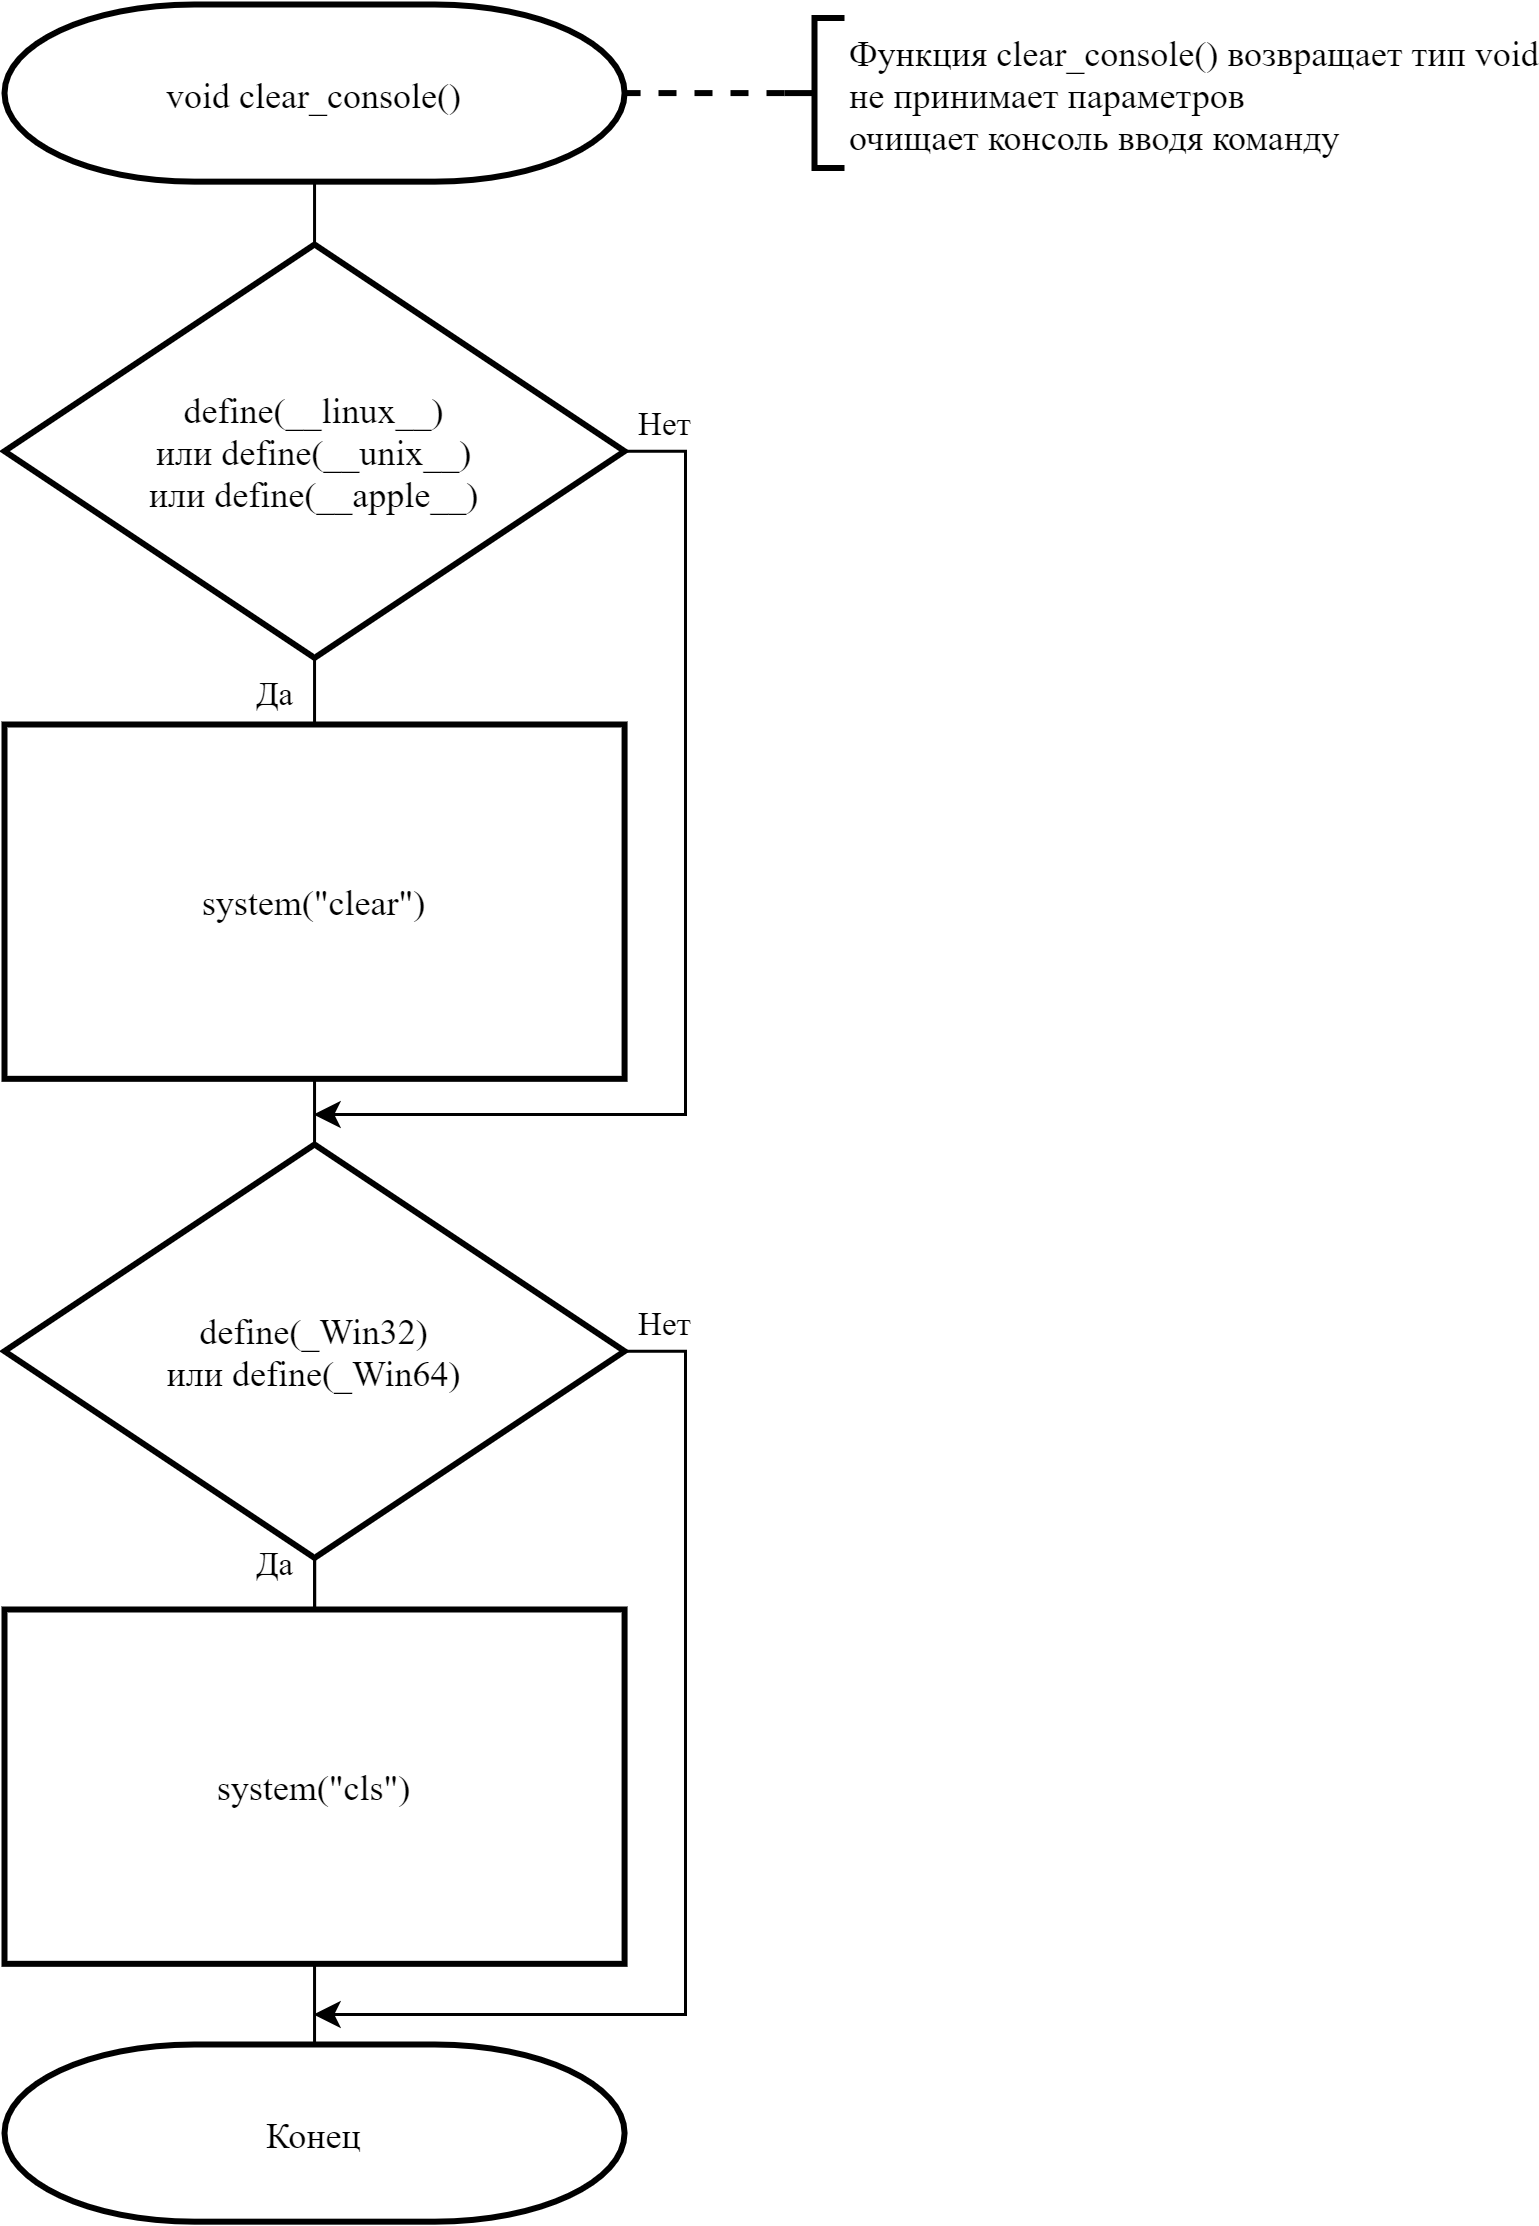
\includegraphics[]{../13/src/my_libs/clearConsole/clearConsole.png}
    }
    \caption{clearConsole()}
    \label{fig:clearConsole}
\end{figure}

\lstinputlisting[
    language=C,
    name=clearConsole.h
]{../13/src/my_libs/clearConsole/clearConsole.h}

\lstinputlisting[
    language=C,
    name=clearConsole.c
]{../13/src/my_libs/clearConsole/clearConsole.c}

\newpage
\subsection{encoding()}

Блок-схема на рисунке \ref{fig:encoding}.

\begin{figure}[h]
    \center{
        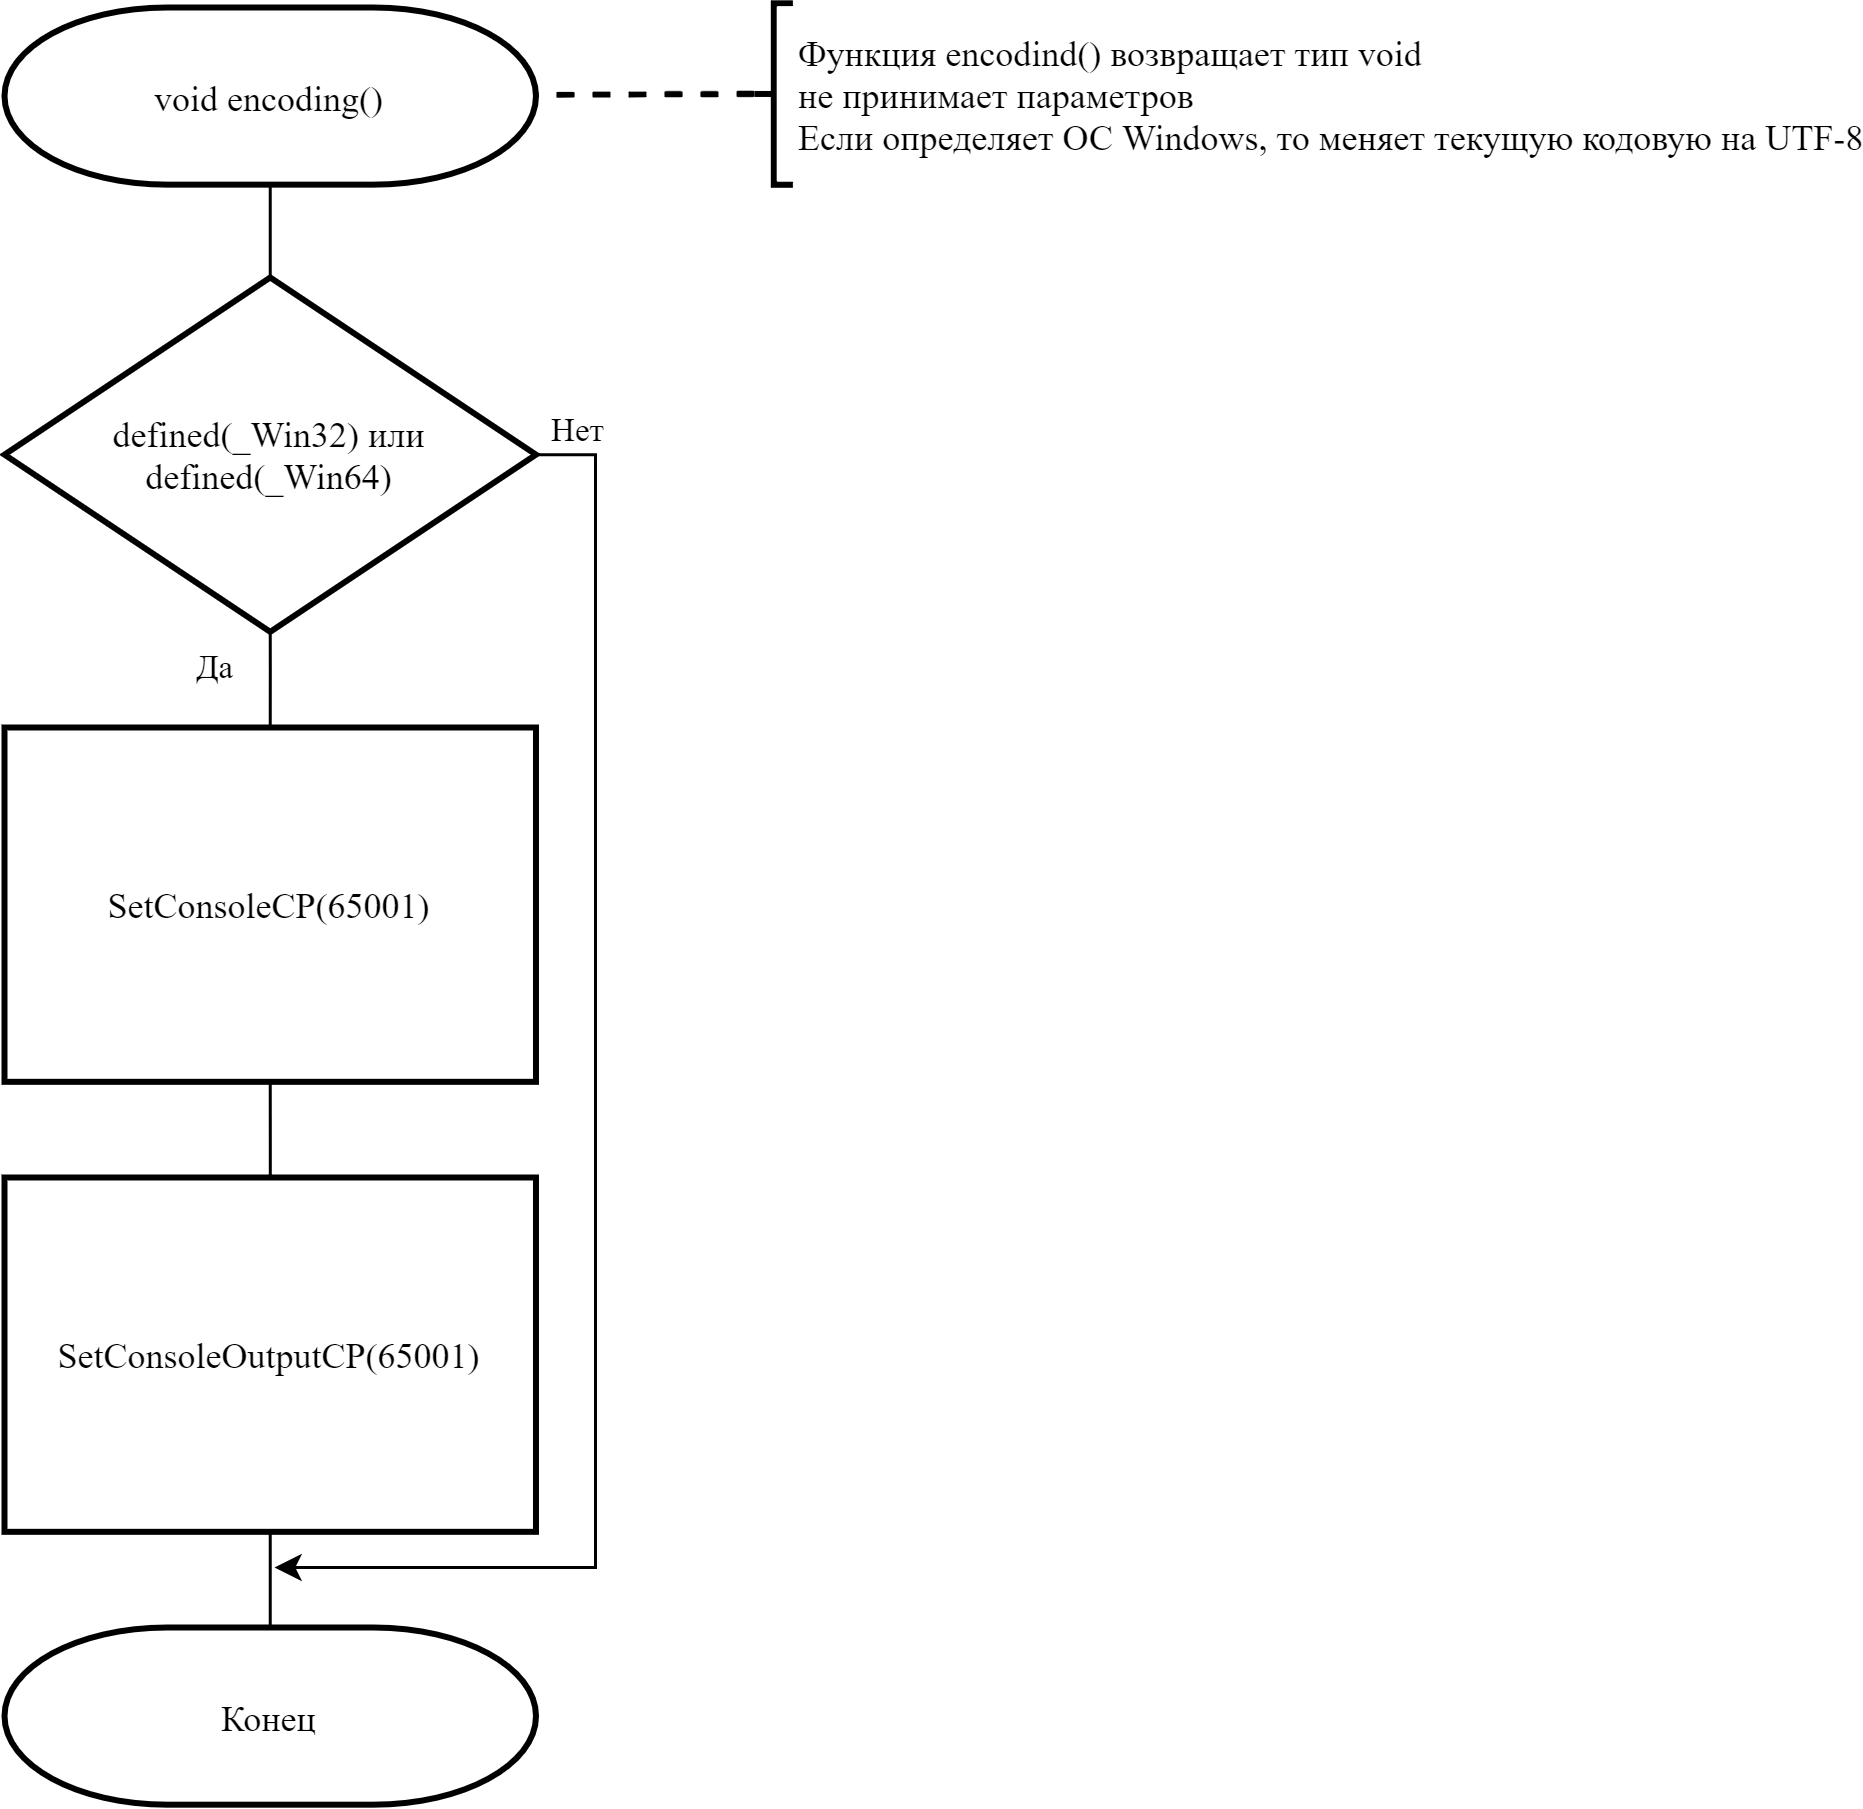
\includegraphics[]{../13/src/my_libs/encoding/encoding.png}
    }
    \caption{encoding()}
    \label{fig:encoding}
\end{figure}

\lstinputlisting[
    language=C,
    name=encoding.h
]{../13/src/my_libs/encoding/encoding.h}

\lstinputlisting[
    language=C,
    name=encoding.c
]{../13/src/my_libs/encoding/encoding.c}

\newpage
\subsection{getch()}

\lstinputlisting[
    language=C,
    name=getch.h
]{../13/src/my_libs/getch/getch.h}

\lstinputlisting[
    language=C,
    name=getch.h
]{../13/src/my_libs/getch/getch.c}

\newpage
\subsection{pause\_console()}

Блок-схема на рисунке \ref{fig:pause_console}.

\begin{figure}[h]
    \center{
        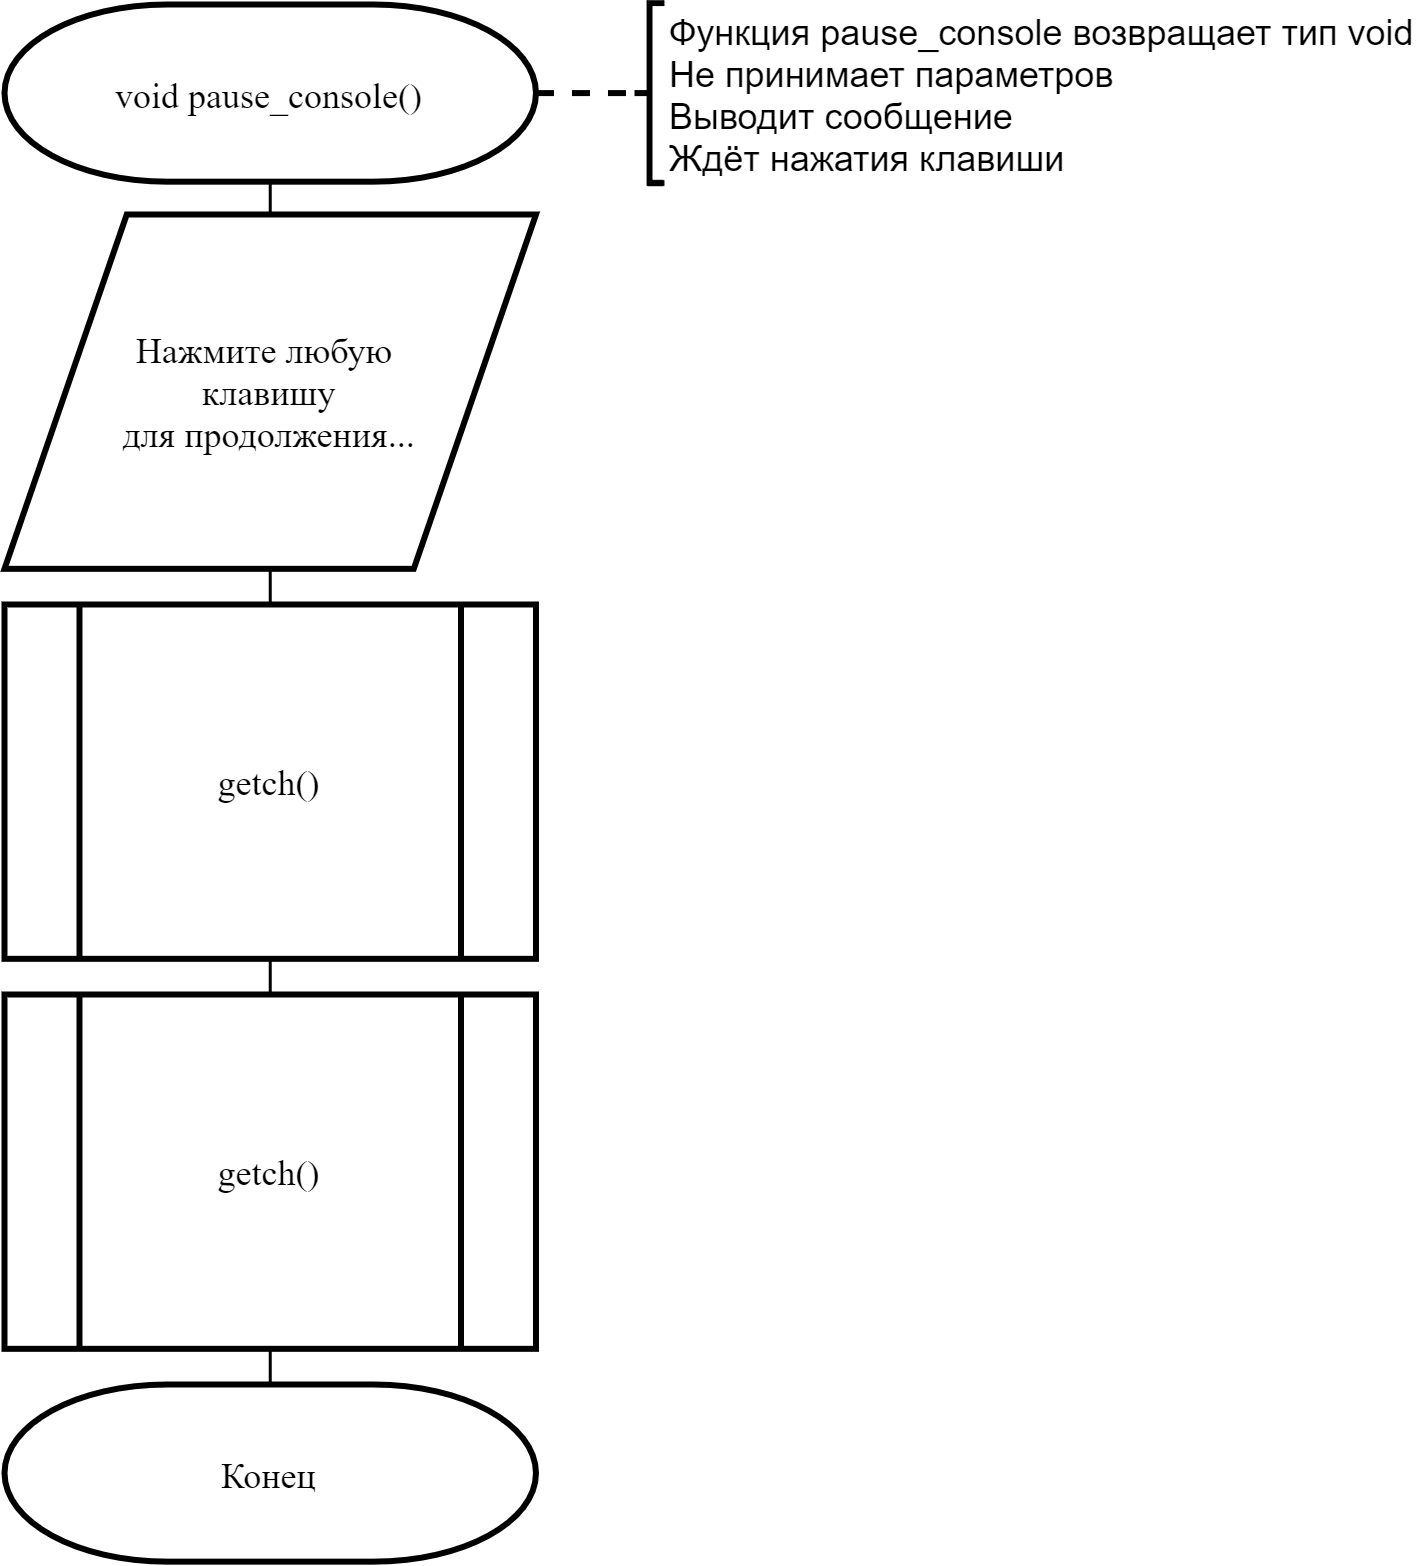
\includegraphics[]{../13/src/my_libs/pause_console/pause_console.png}
    }
    \caption{pause\_console()}
    \label{fig:pause_console}
\end{figure}

\lstinputlisting[
    language=C,
    name=pause\_console.h
]{../13/src/my_libs/pause_console/pause_console.h}

\lstinputlisting[
    language=C,
    name=pause\_console.c
]{../13/src/my_libs/pause_console/pause_console.c}

\newpage

\subsubsection{lab()}

Блок-схема на рисунке \ref{fig:lab}.

\begin{figure}[h]
    \center{
        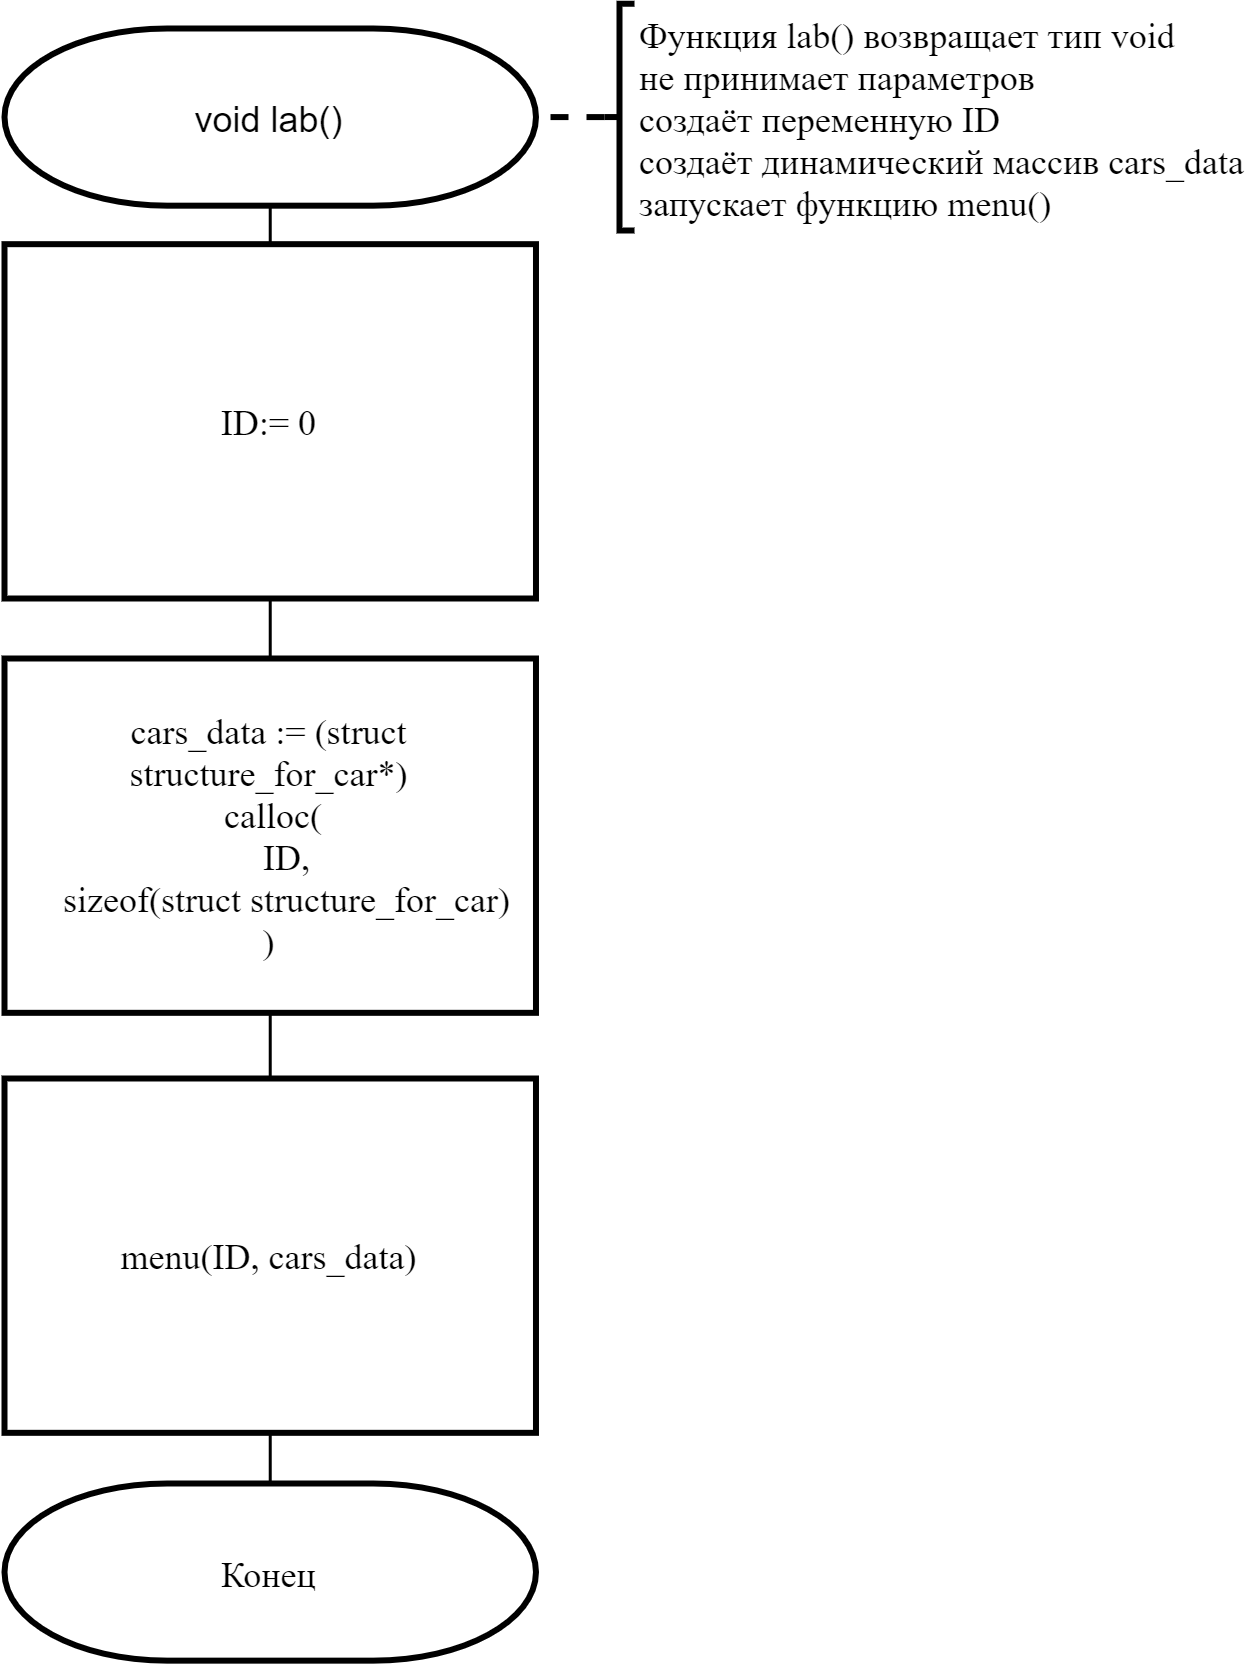
\includegraphics[]{../13/src/lab/lab.png}
    }
    \caption{lab()}
    \label{fig:lab}
\end{figure}

\lstinputlisting[
    language=C,
    name=lab.h
]{../13/src/lab/lab.h}

\lstinputlisting[
    language=C,
    name=lab.c
]{../13/src/lab/lab.c}

\newpage
\subsubsection{menu()}

Блок-схема на рисунке \ref{fig:menu}.

\begin{figure}[p]
    \center{
        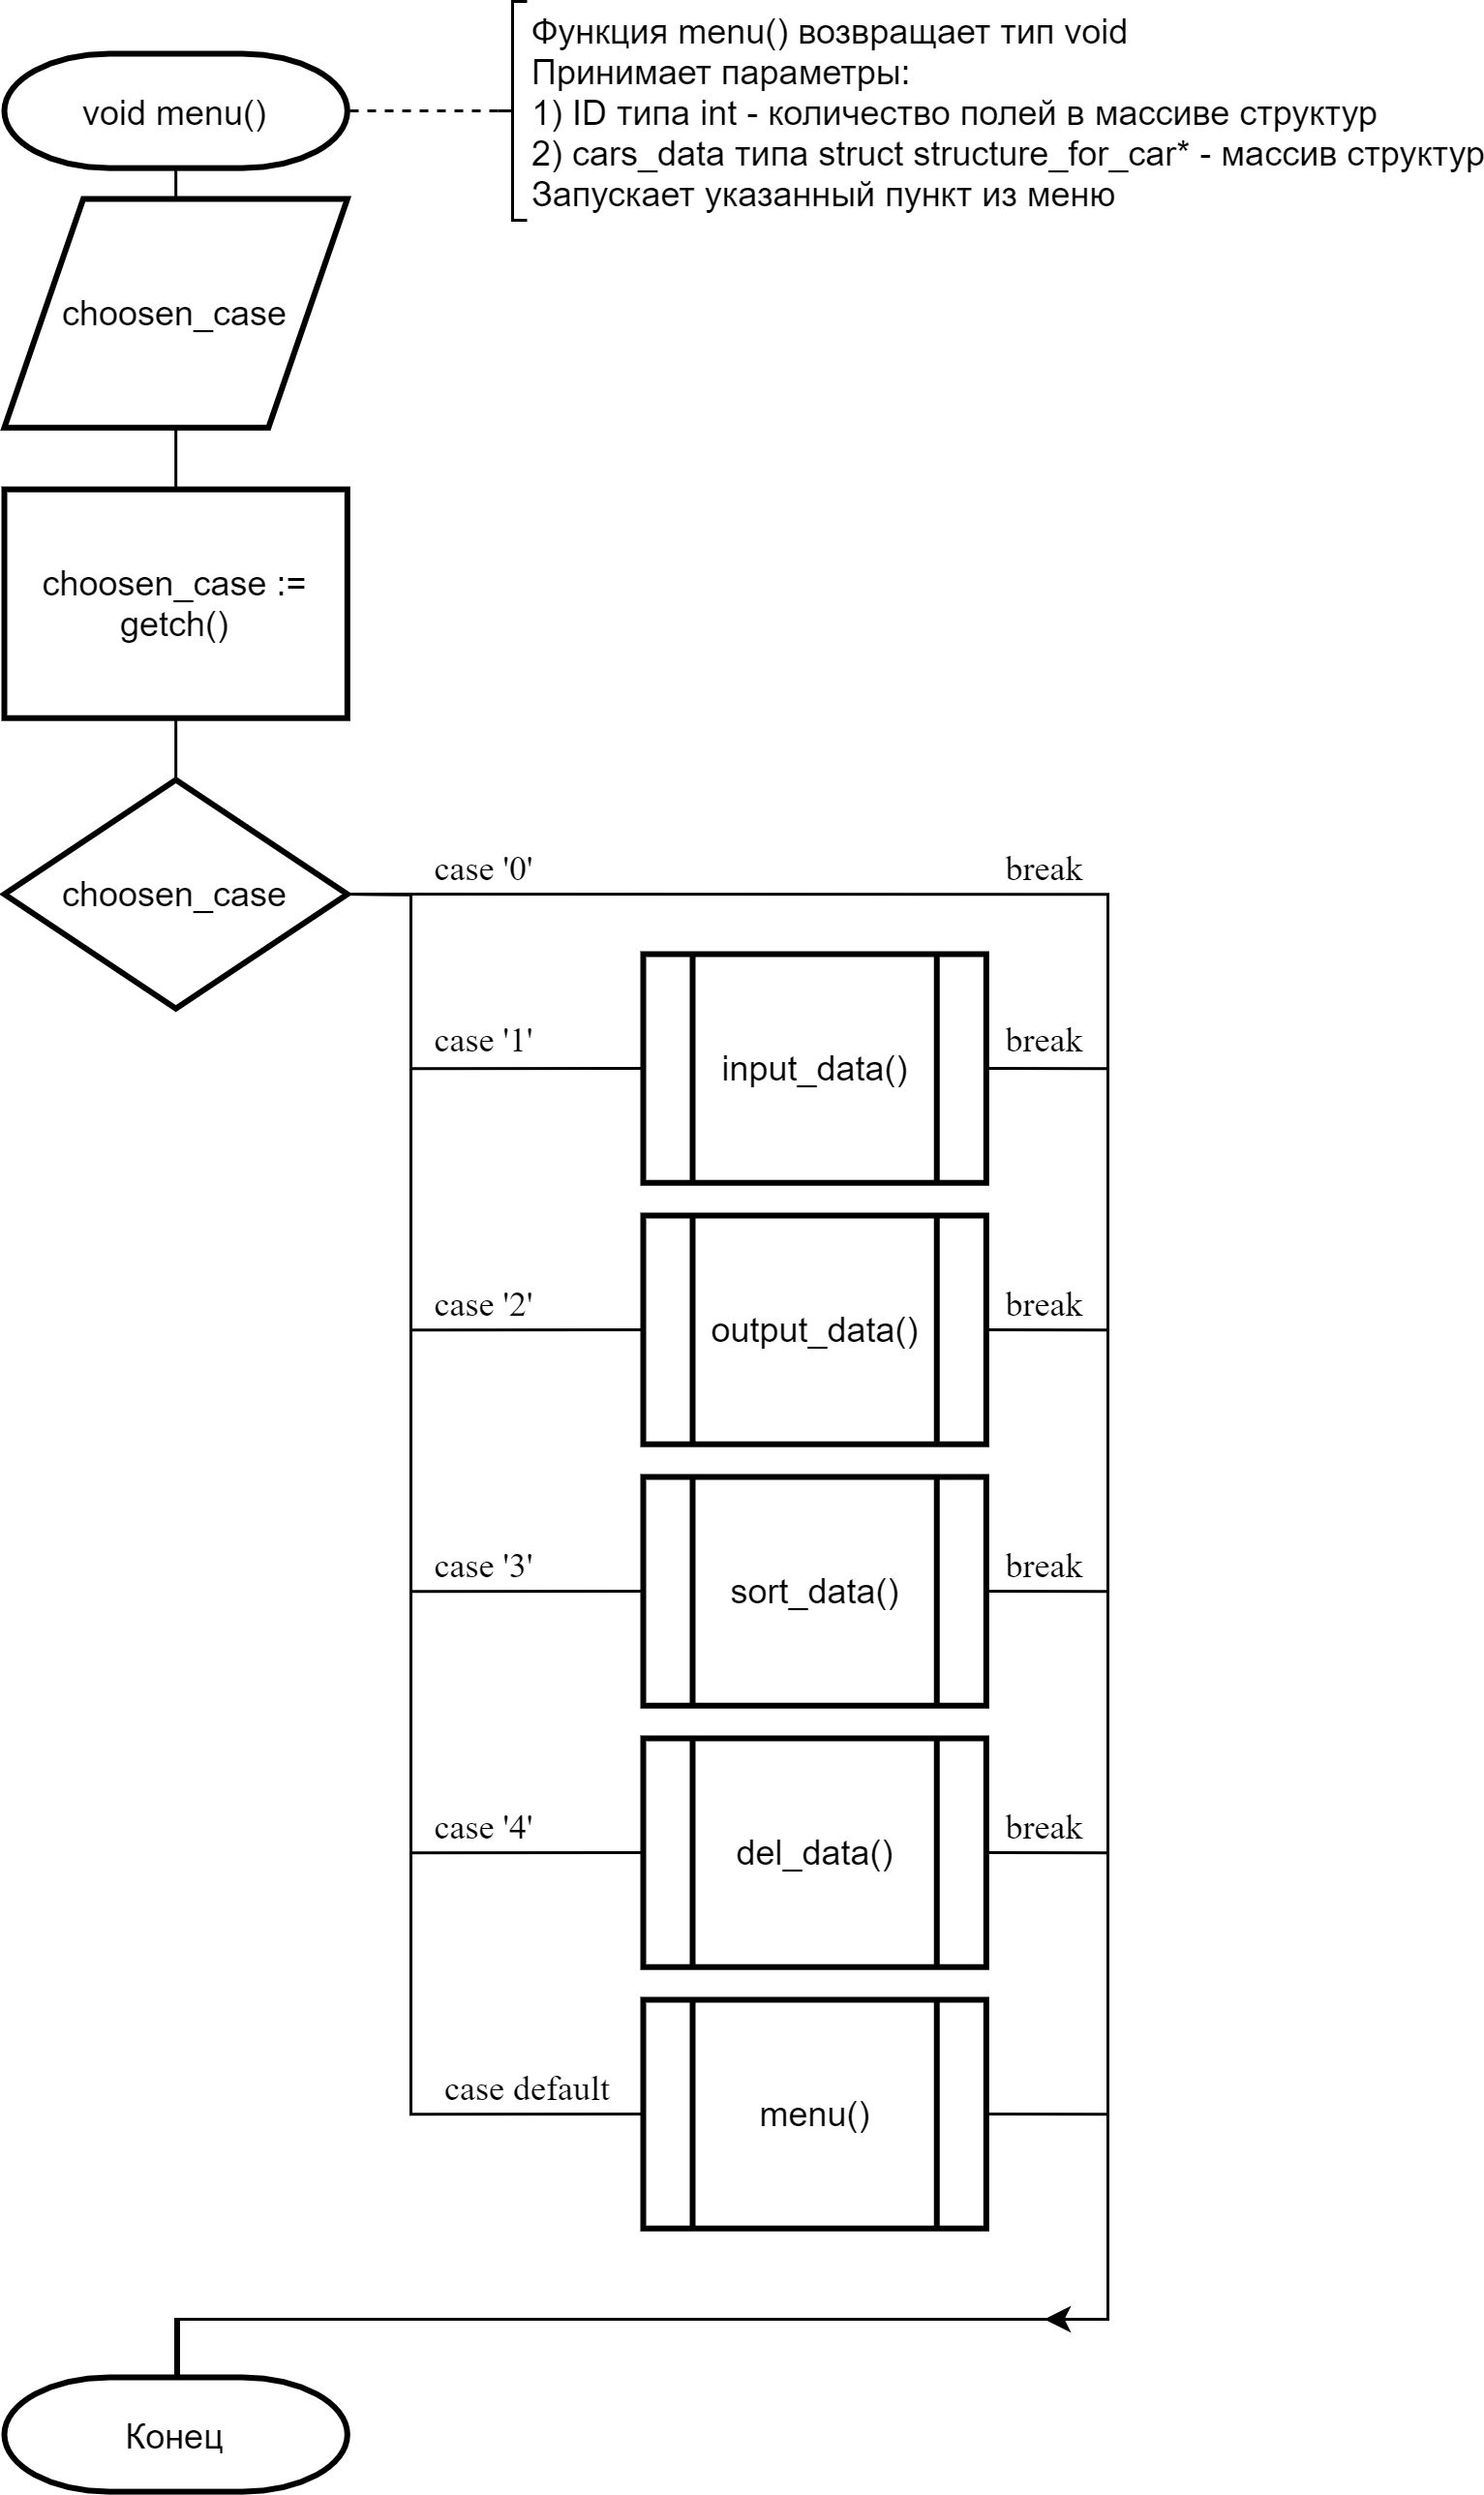
\includegraphics[]{../13/src/lab/menu/menu.png}
    }
    \caption{menu()}
    \label{fig:menu}
\end{figure}

\lstinputlisting[
    language=C,
    name=menu.h
]{../13/src/lab/menu/menu.h}

\lstinputlisting[
    language=C,
    name=menu.c
]{../13/src/lab/menu/menu.c}

\newpage
\subsection{del\_data()}

Блок-схема на рисунке \ref{fig:del_data}.

\begin{figure}[p]
    \center{
        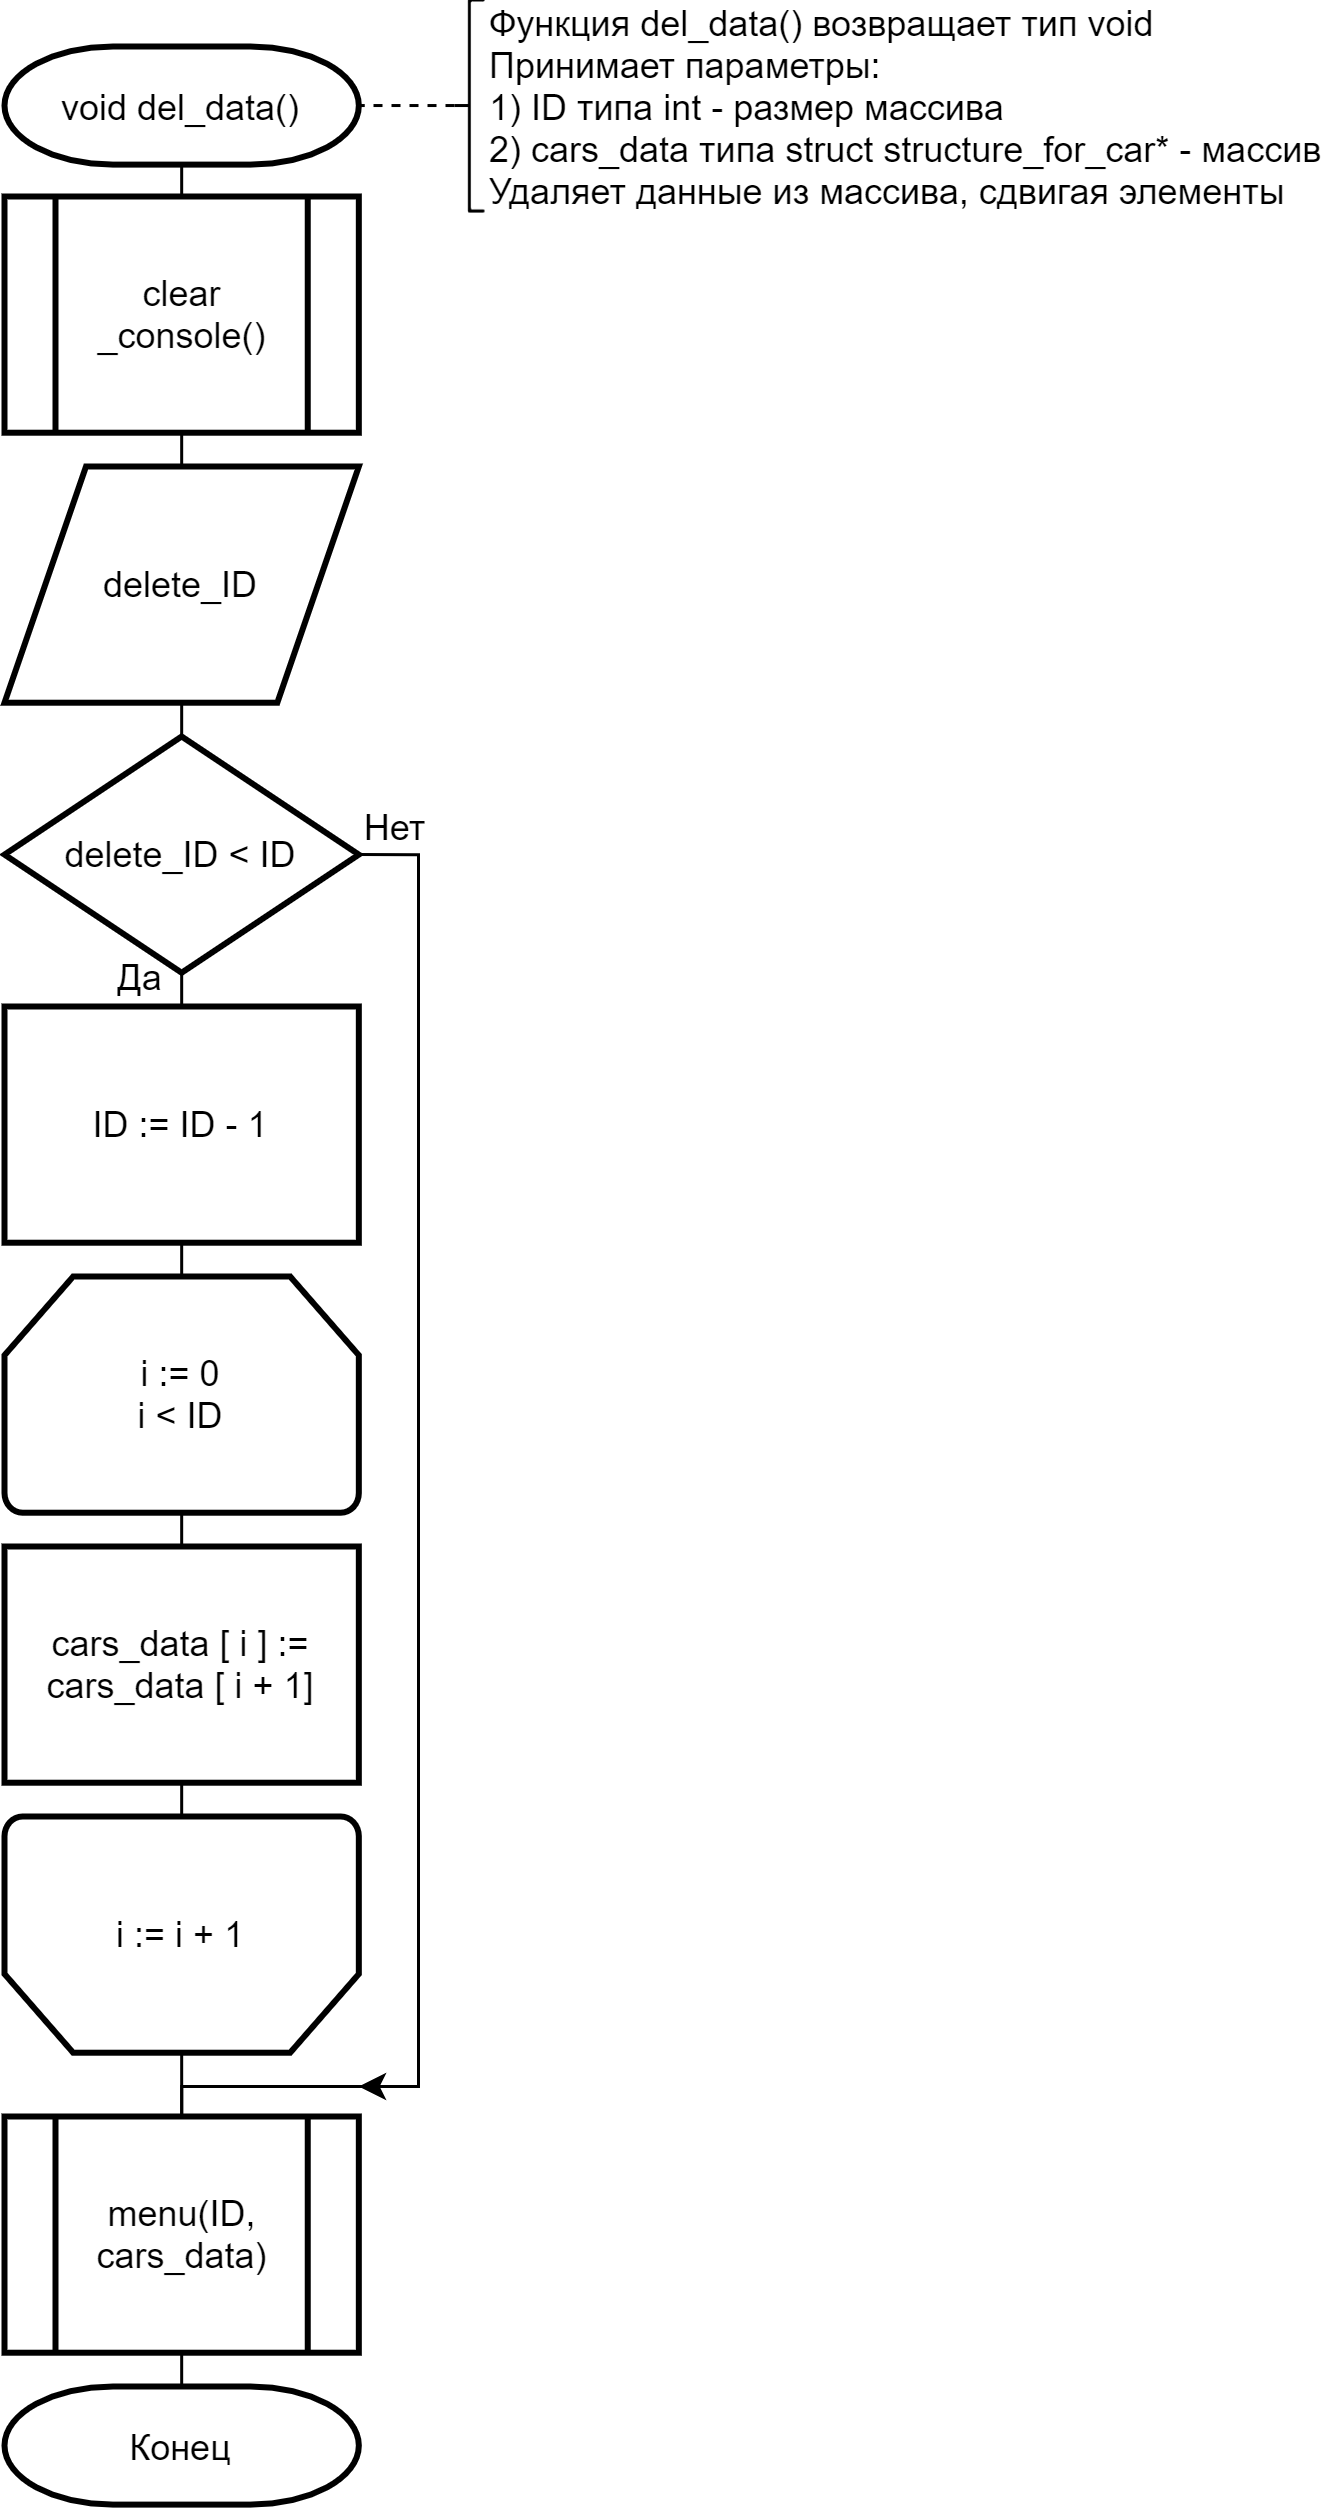
\includegraphics[]{../13/src/lab/menu/del_data/del_data.png}
    }
    \caption{del\_data()}
    \label{fig:del_data}
\end{figure}

\lstinputlisting[
    language=C,
    name=del\_data.h
]{../13/src/lab/menu/del_data/del_data.h}

\lstinputlisting[
    language=C,
    name=del\_data.c
]{../13/src/lab/menu/del_data/del_data.c}

\newpage
\subsubsection{input\_data()}

Блок-схема на рисунке \ref{fig:input_data}.

\begin{figure}[p]
    \center{
        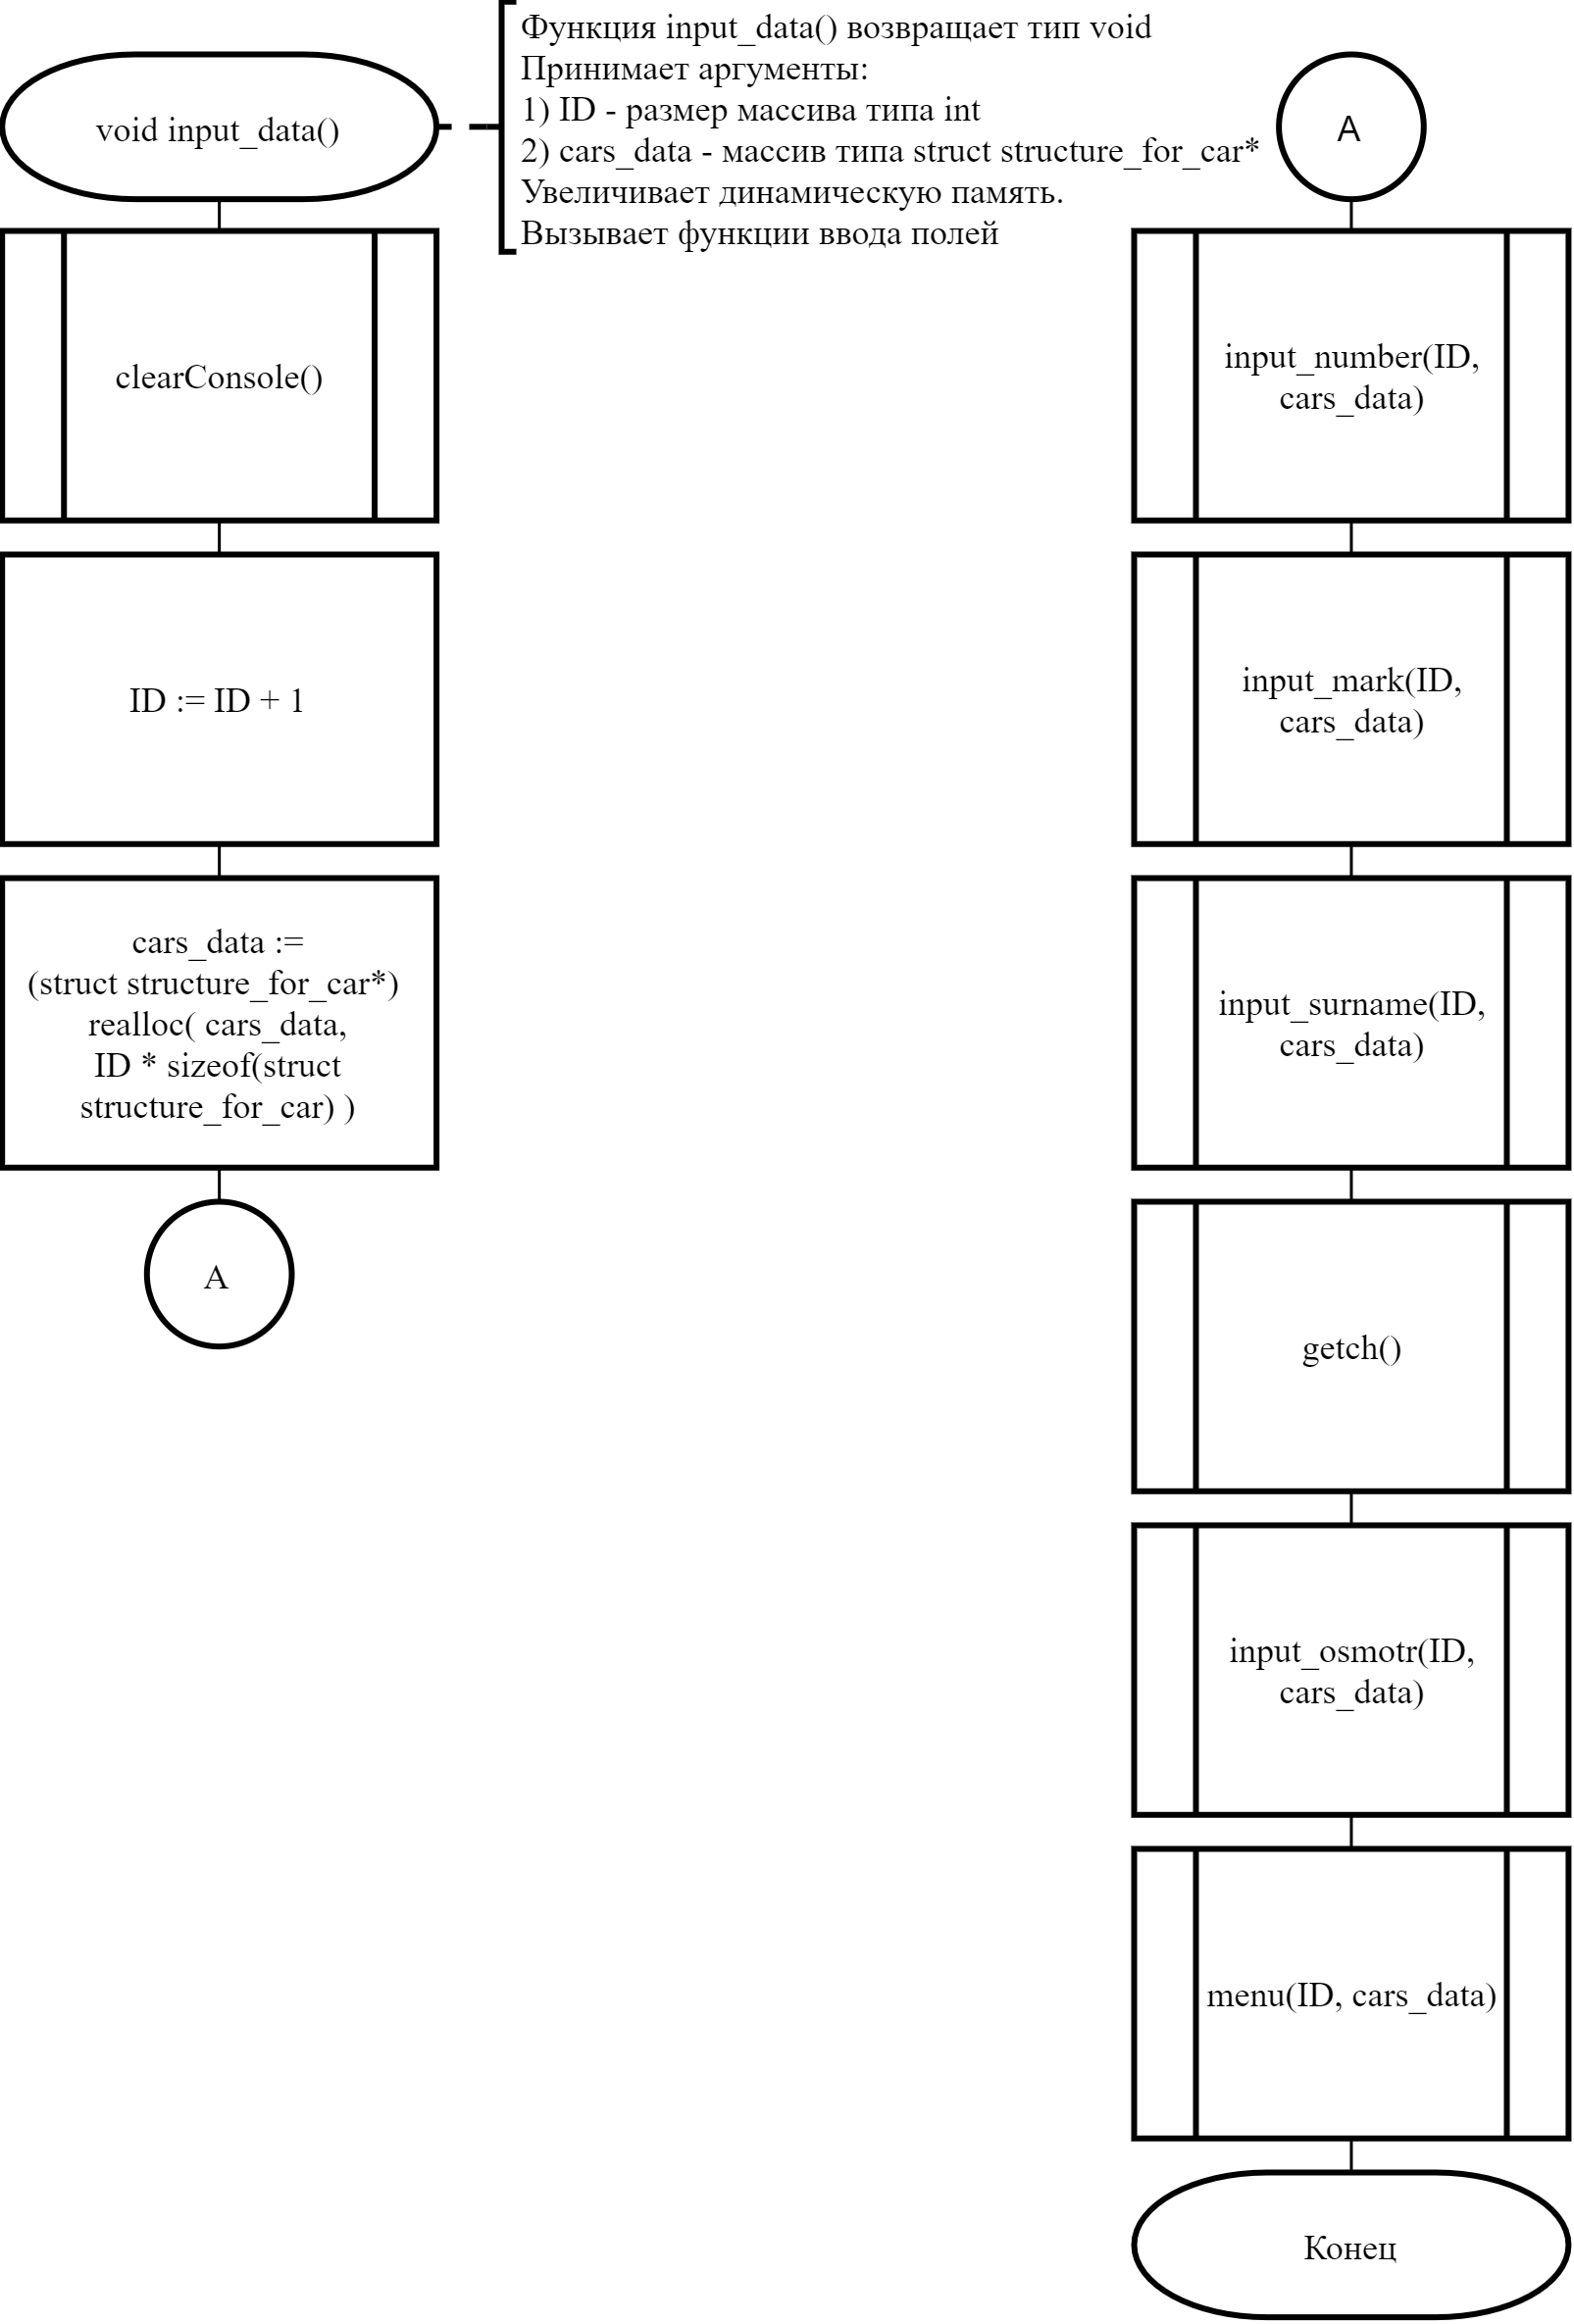
\includegraphics[width=16cm]{../13/src/lab/menu/input_data/input_data.png}
    }
    \caption{input\_data()}
    \label{fig:input_data}
\end{figure}

\lstinputlisting[
    language=C,
    name=input\_data.h
]{../13/src/lab/menu/input_data/input_data.h}

\lstinputlisting[
    language=C,
    name=input\_data.c
]{../13/src/lab/menu/input_data/input_data.c}

\newpage
\subsection{out\_data()}

Блок-схема на рисунке \ref{fig:out_data}.

\begin{figure}[p]
    \center{
        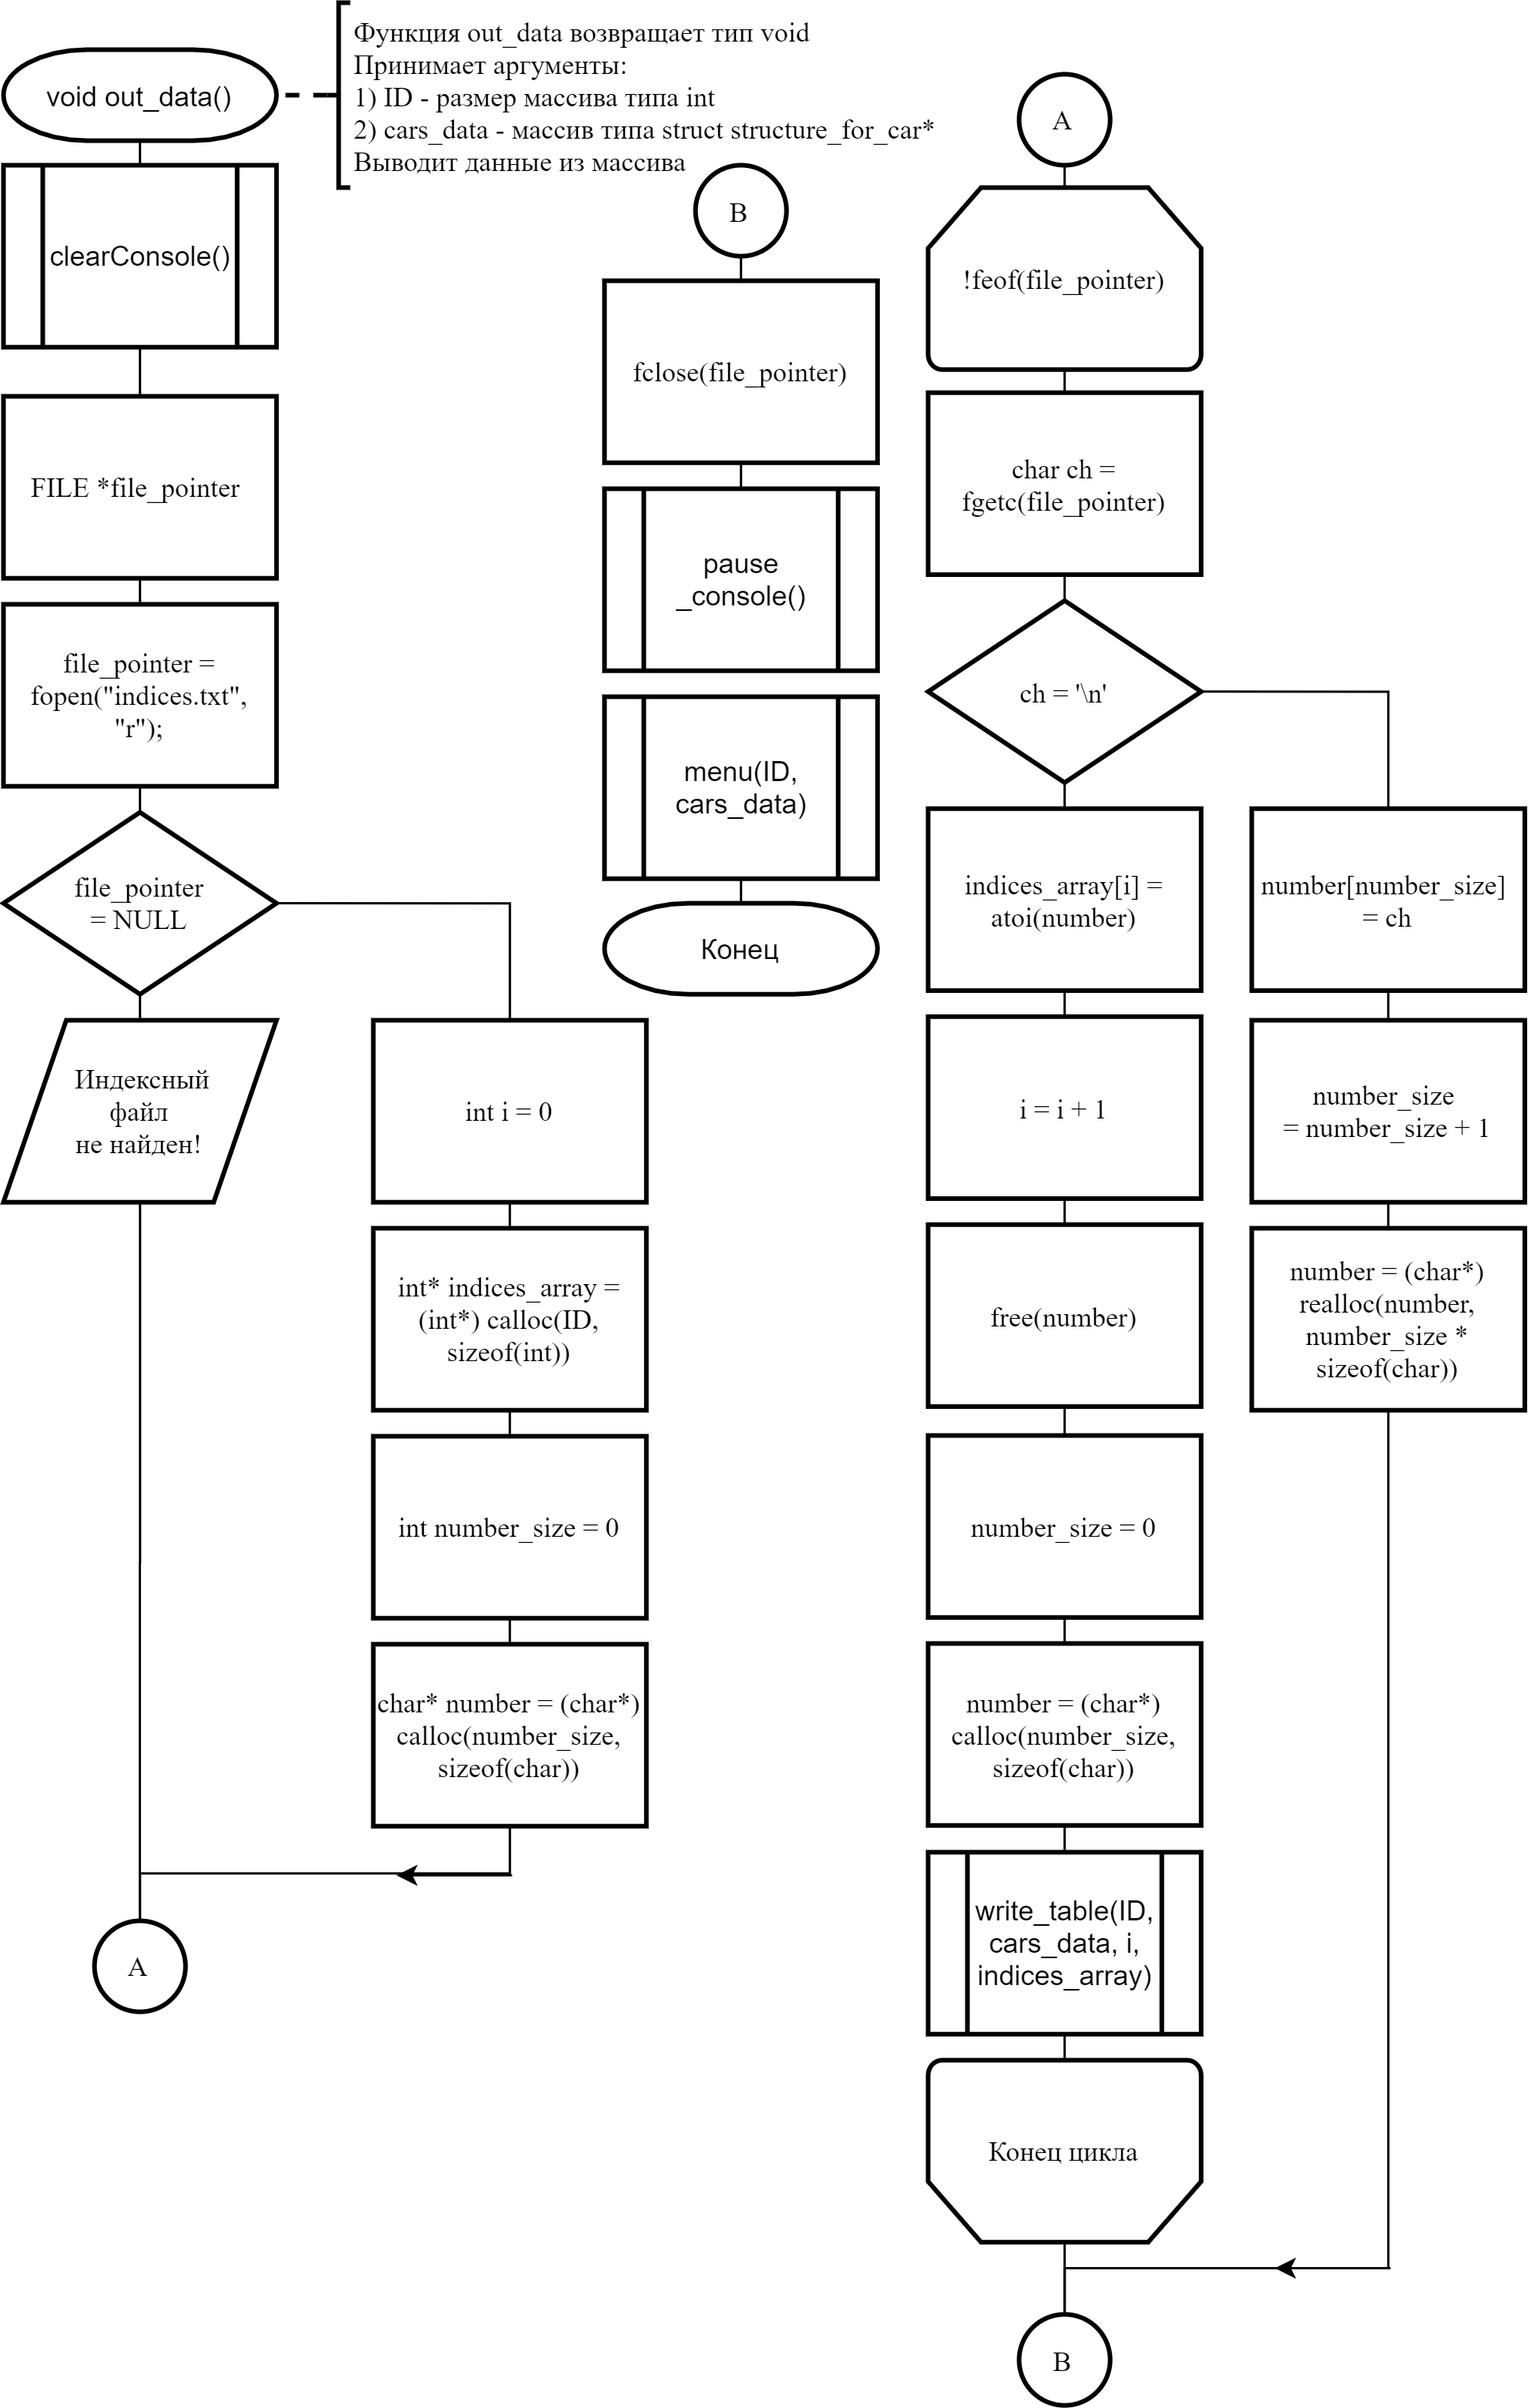
\includegraphics[]{../13/src/lab/menu/out_data/out_data.png}
    }
    \caption{out\_data()}
    \label{fig:out_data}
\end{figure}

\lstinputlisting[
    language=C,
    name=out\_data.h
]{../13/src/lab/menu/out_data/out_data.h}

\lstinputlisting[
    language=C,
    name=out\_data.c
]{../13/src/lab/menu/out_data/out_data.c}

\newpage
\subsubsection{sort\_data()}

Блок-схема на рисунке \ref{fig:sort_data}.

\begin{figure}[p]
    \center{
        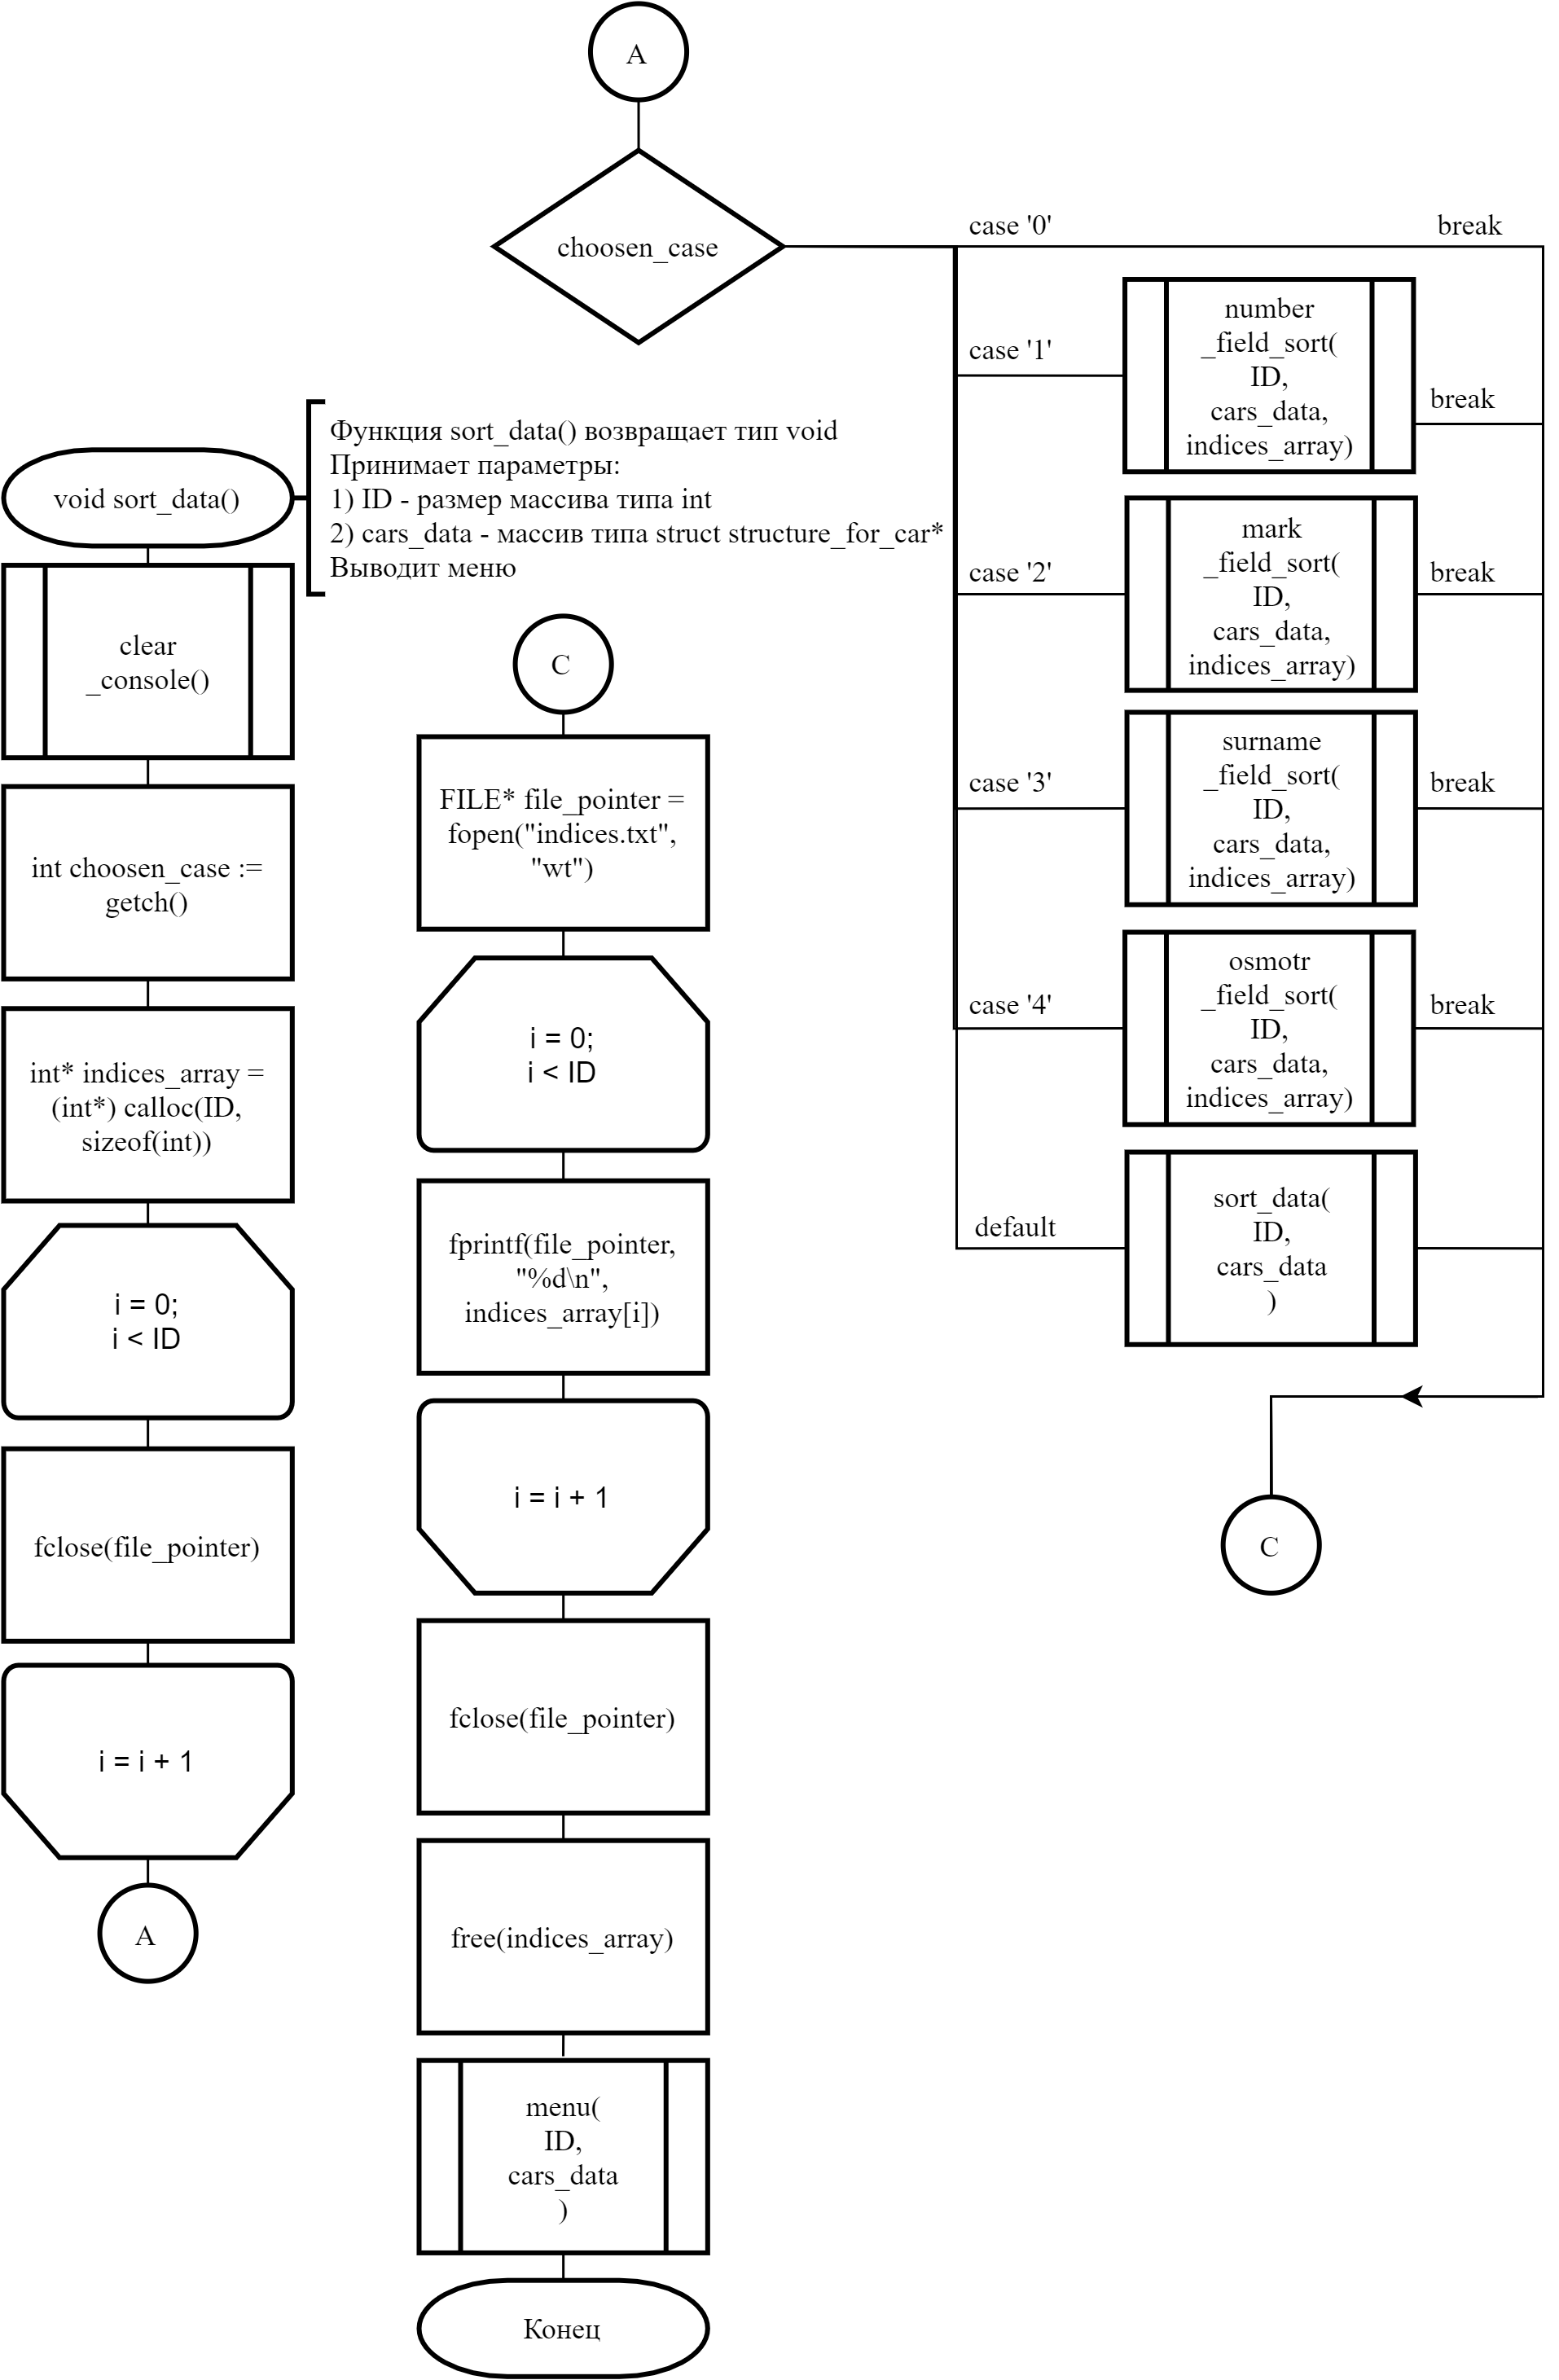
\includegraphics[]{../13/src/lab/menu/sort_data/sort_data.png}
    }
    \caption{sort\_data()}
    \label{fig:sort_data}
\end{figure}

\lstinputlisting[
    language=C,
    name=sort\_data.h
]{../13/src/lab/menu/sort_data/sort_data.h}

\lstinputlisting[
    language=C,
    name=sort\_data.c
]{../13/src/lab/menu/sort_data/sort_data.c}

\newpage

\subsection{sort\_data\_by\_mark\_field()}

Блок-схема на рисунке \ref{fig:sort_data_by_mark_field}.

\begin{figure}[p]
    \center{
        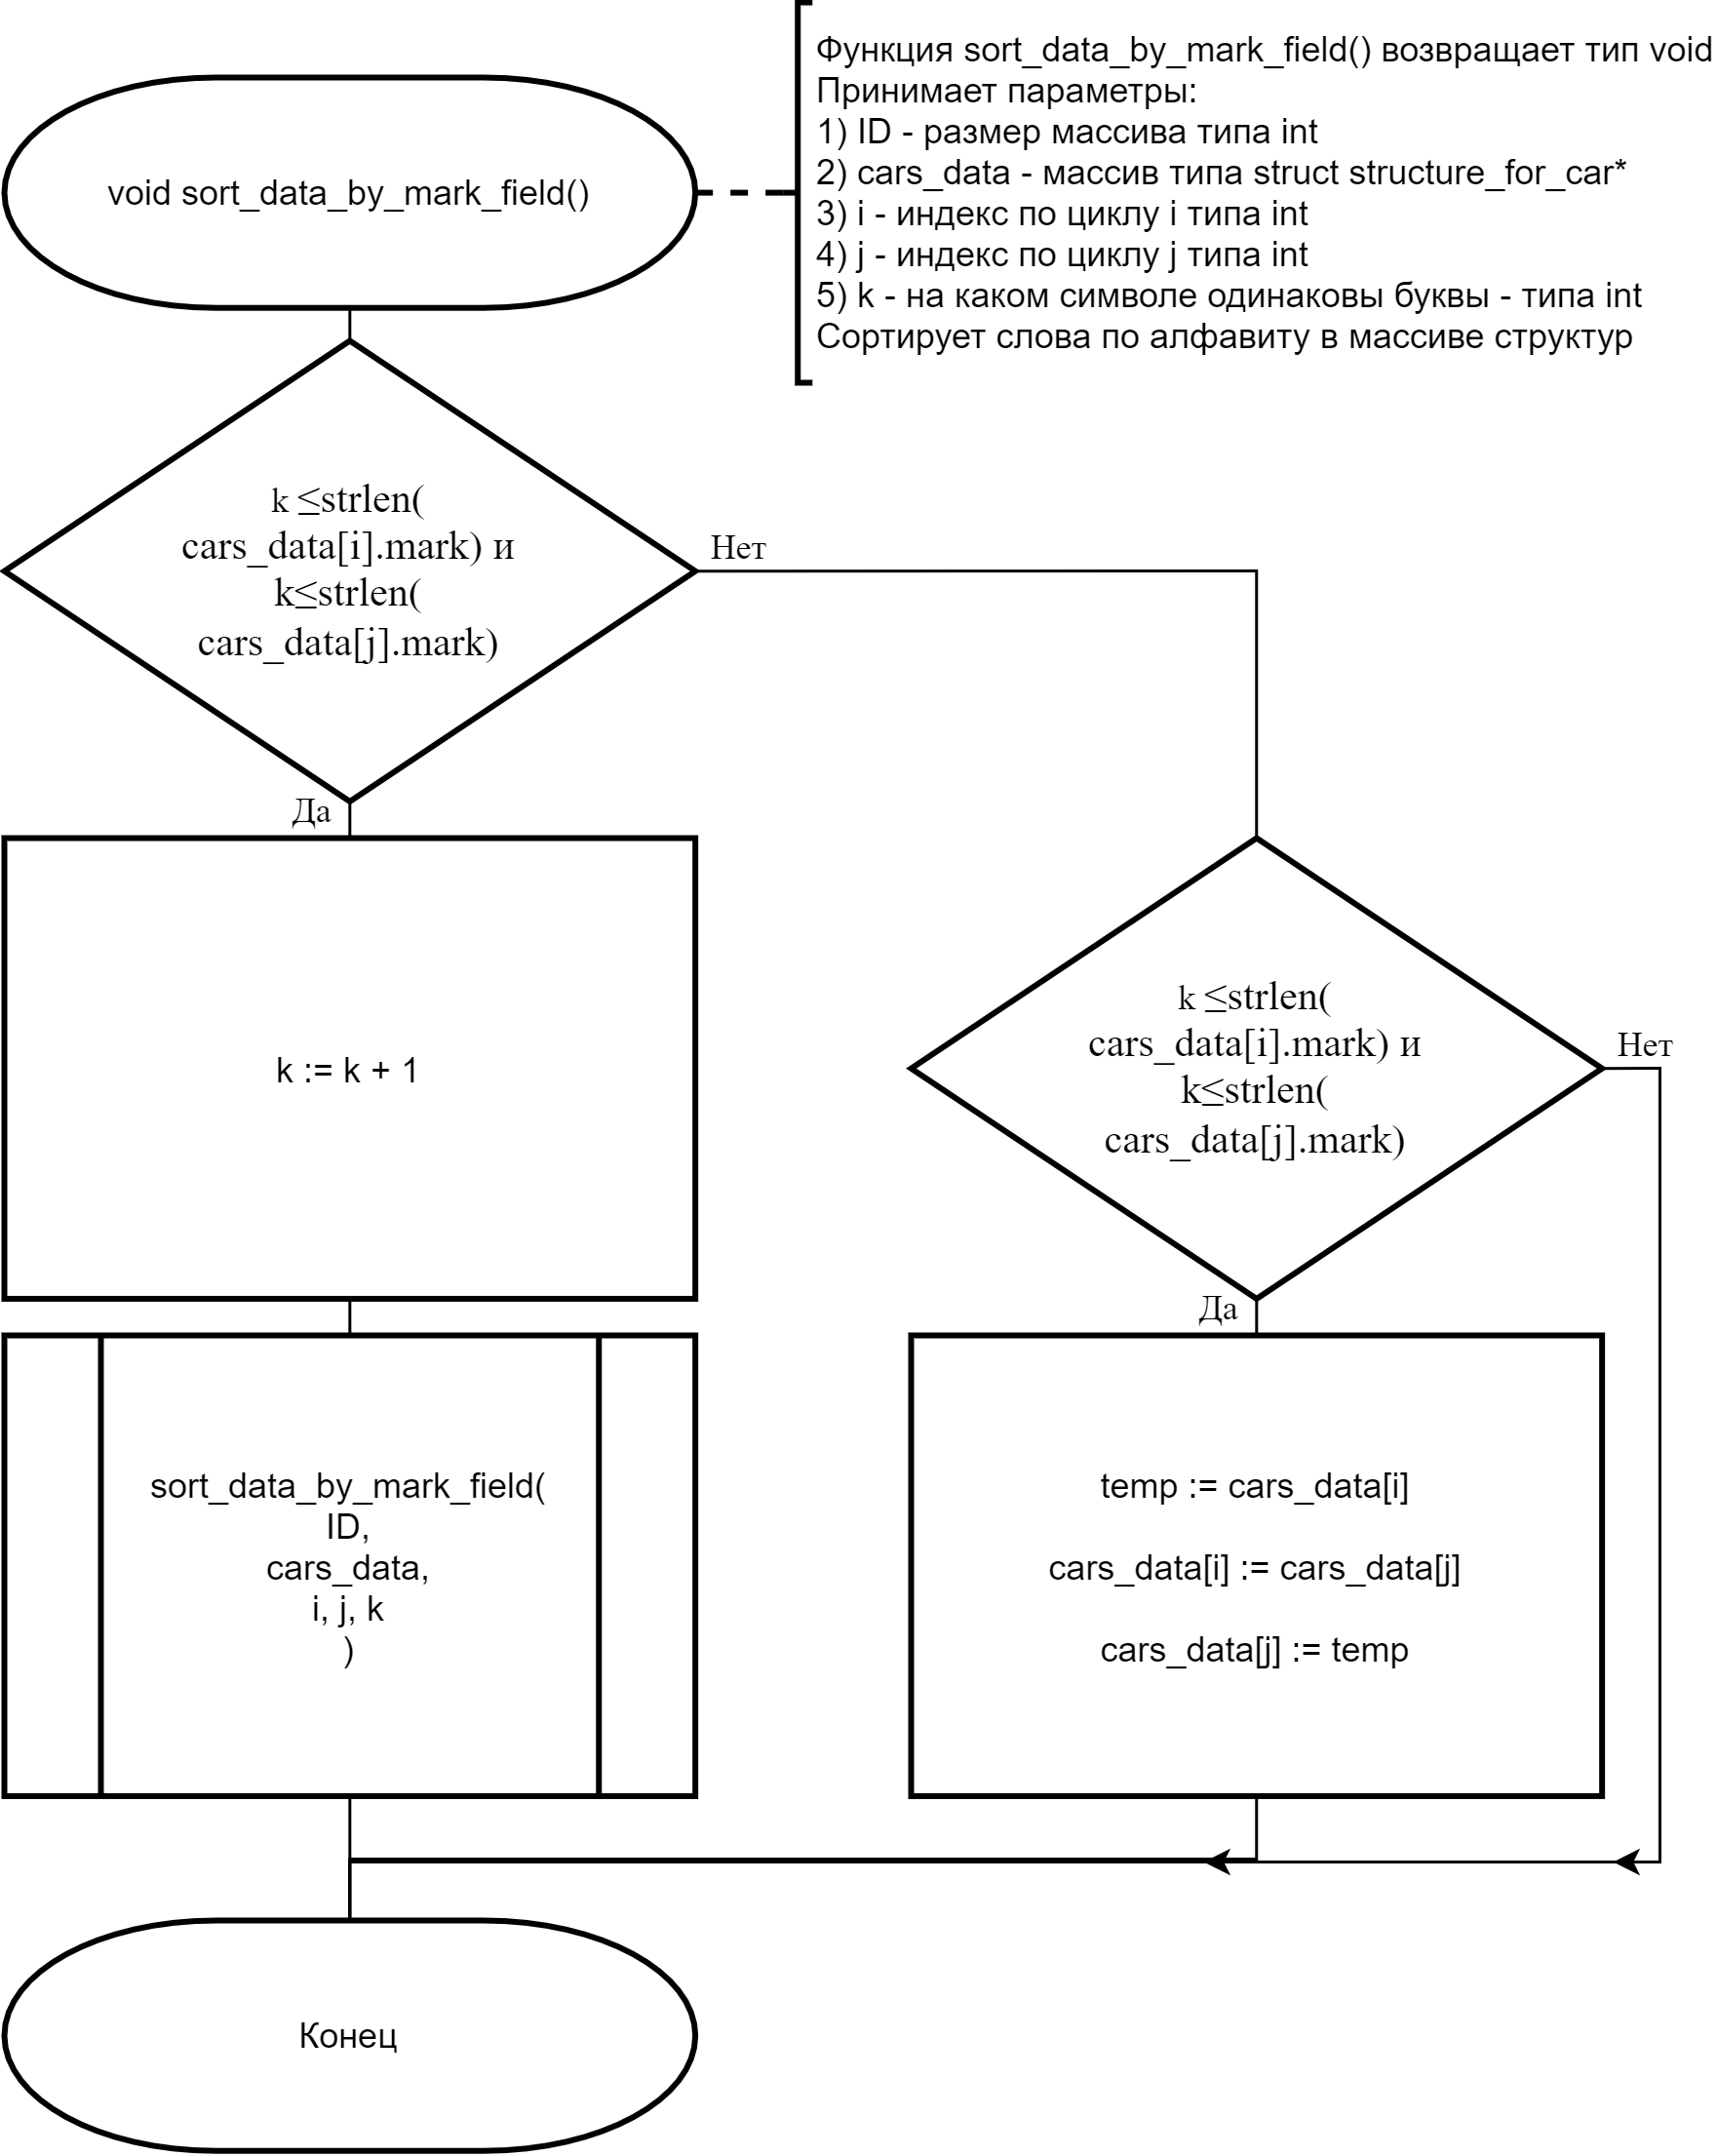
\includegraphics[]{../13/src/lab/menu/sort_data/get_sorted_array/sort_data_by_mark_field/sort_data_by_mark_field.png}
    }
    \caption{sort\_data\_by\_mark\_field()}
    \label{fig:sort_data_by_mark_field}
\end{figure}

\lstinputlisting[
	language=C,
	name=sort\_data\_by\_mark\_field.h
]{../13/src/lab/menu/sort_data/get_sorted_array/sort_data_by_mark_field/sort_data_by_mark_field.h}

\lstinputlisting[
	language=C,
	name=sort\_data\_by\_mark\_field.c
]{../13/src/lab/menu/sort_data/get_sorted_array/sort_data_by_mark_field/sort_data_by_mark_field.c}

\newpage
\subsection{sort\_data\_by\_osmotr\_field()}

\lstinputlisting[
	language=C,
	name=sort\_data\_by\_osmotr\_field.h
]{../13/src/lab/menu/sort_data/sort_data_by_osmotr_field/sort_data_by_osmotr_field.h}

\lstinputlisting[
	language=C,
	name=sort\_data\_by\_osmotr\_field.c
]{../13/src/lab/menu/sort_data/sort_data_by_osmotr_field/sort_data_by_osmotr_field.c}

\newpage
\subsection{sort\_data\_by\_surname\_field()}

Блок-схема на рисунке \ref{fig:sort_data_by_surname_field}.

\begin{figure}[p]
    \center{
        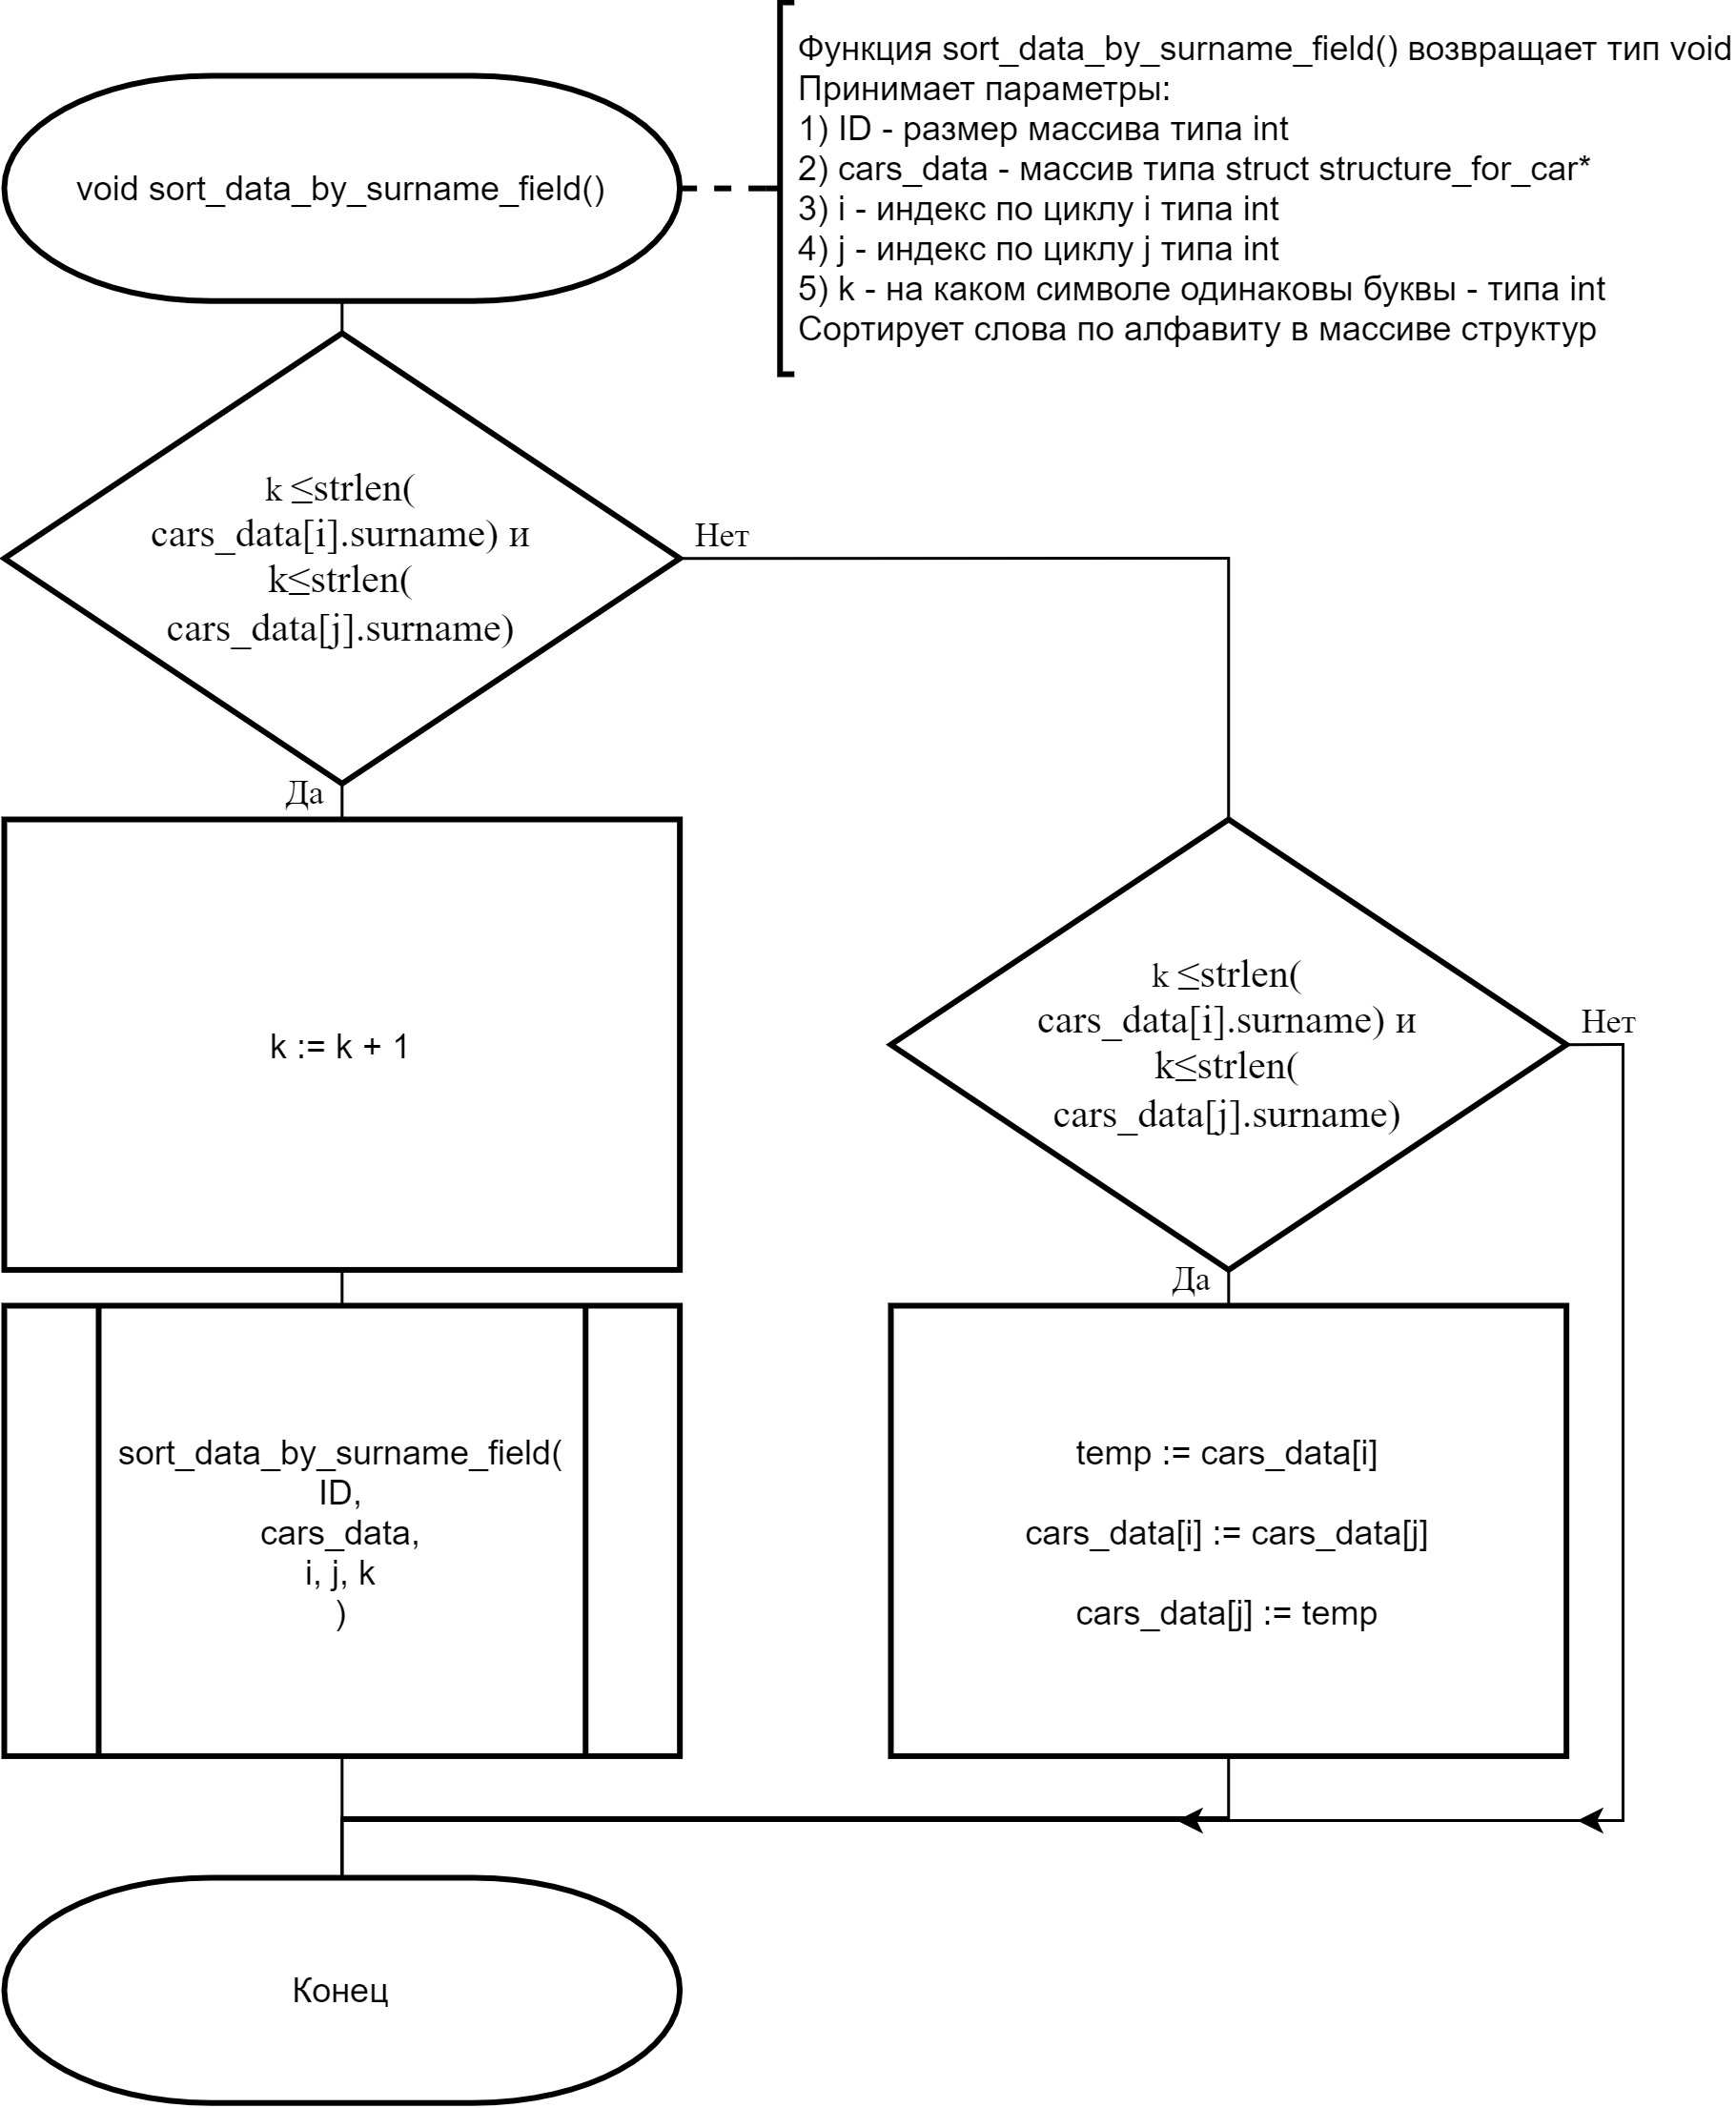
\includegraphics[]{../13/src/lab/menu/sort_data/sort_data_by_surname_field/sort_data_by_surname_field.png}
    }
    \caption{sort\_data\_by\_surname\_field()}
    \label{fig:sort_data_by_surname_field}
\end{figure}

\lstinputlisting[
	language=C,
	name=sort\_data\_by\_surname\_field.h
]{../13/src/lab/menu/sort_data/sort_data_by_surname_field/sort_data_by_surname_field.h}

\lstinputlisting[
	language=C,
	name=sort\_data\_by\_surname\_field.c
]{../13/src/lab/menu/sort_data/sort_data_by_surname_field/sort_data_by_surname_field.c}

\newpage
\subsection{sort\_data\_in\_number\_field()}

Блок-схема на рисунке \ref{fig:sort_data_in_number_field}.

\begin{figure}[p]
    \center{
        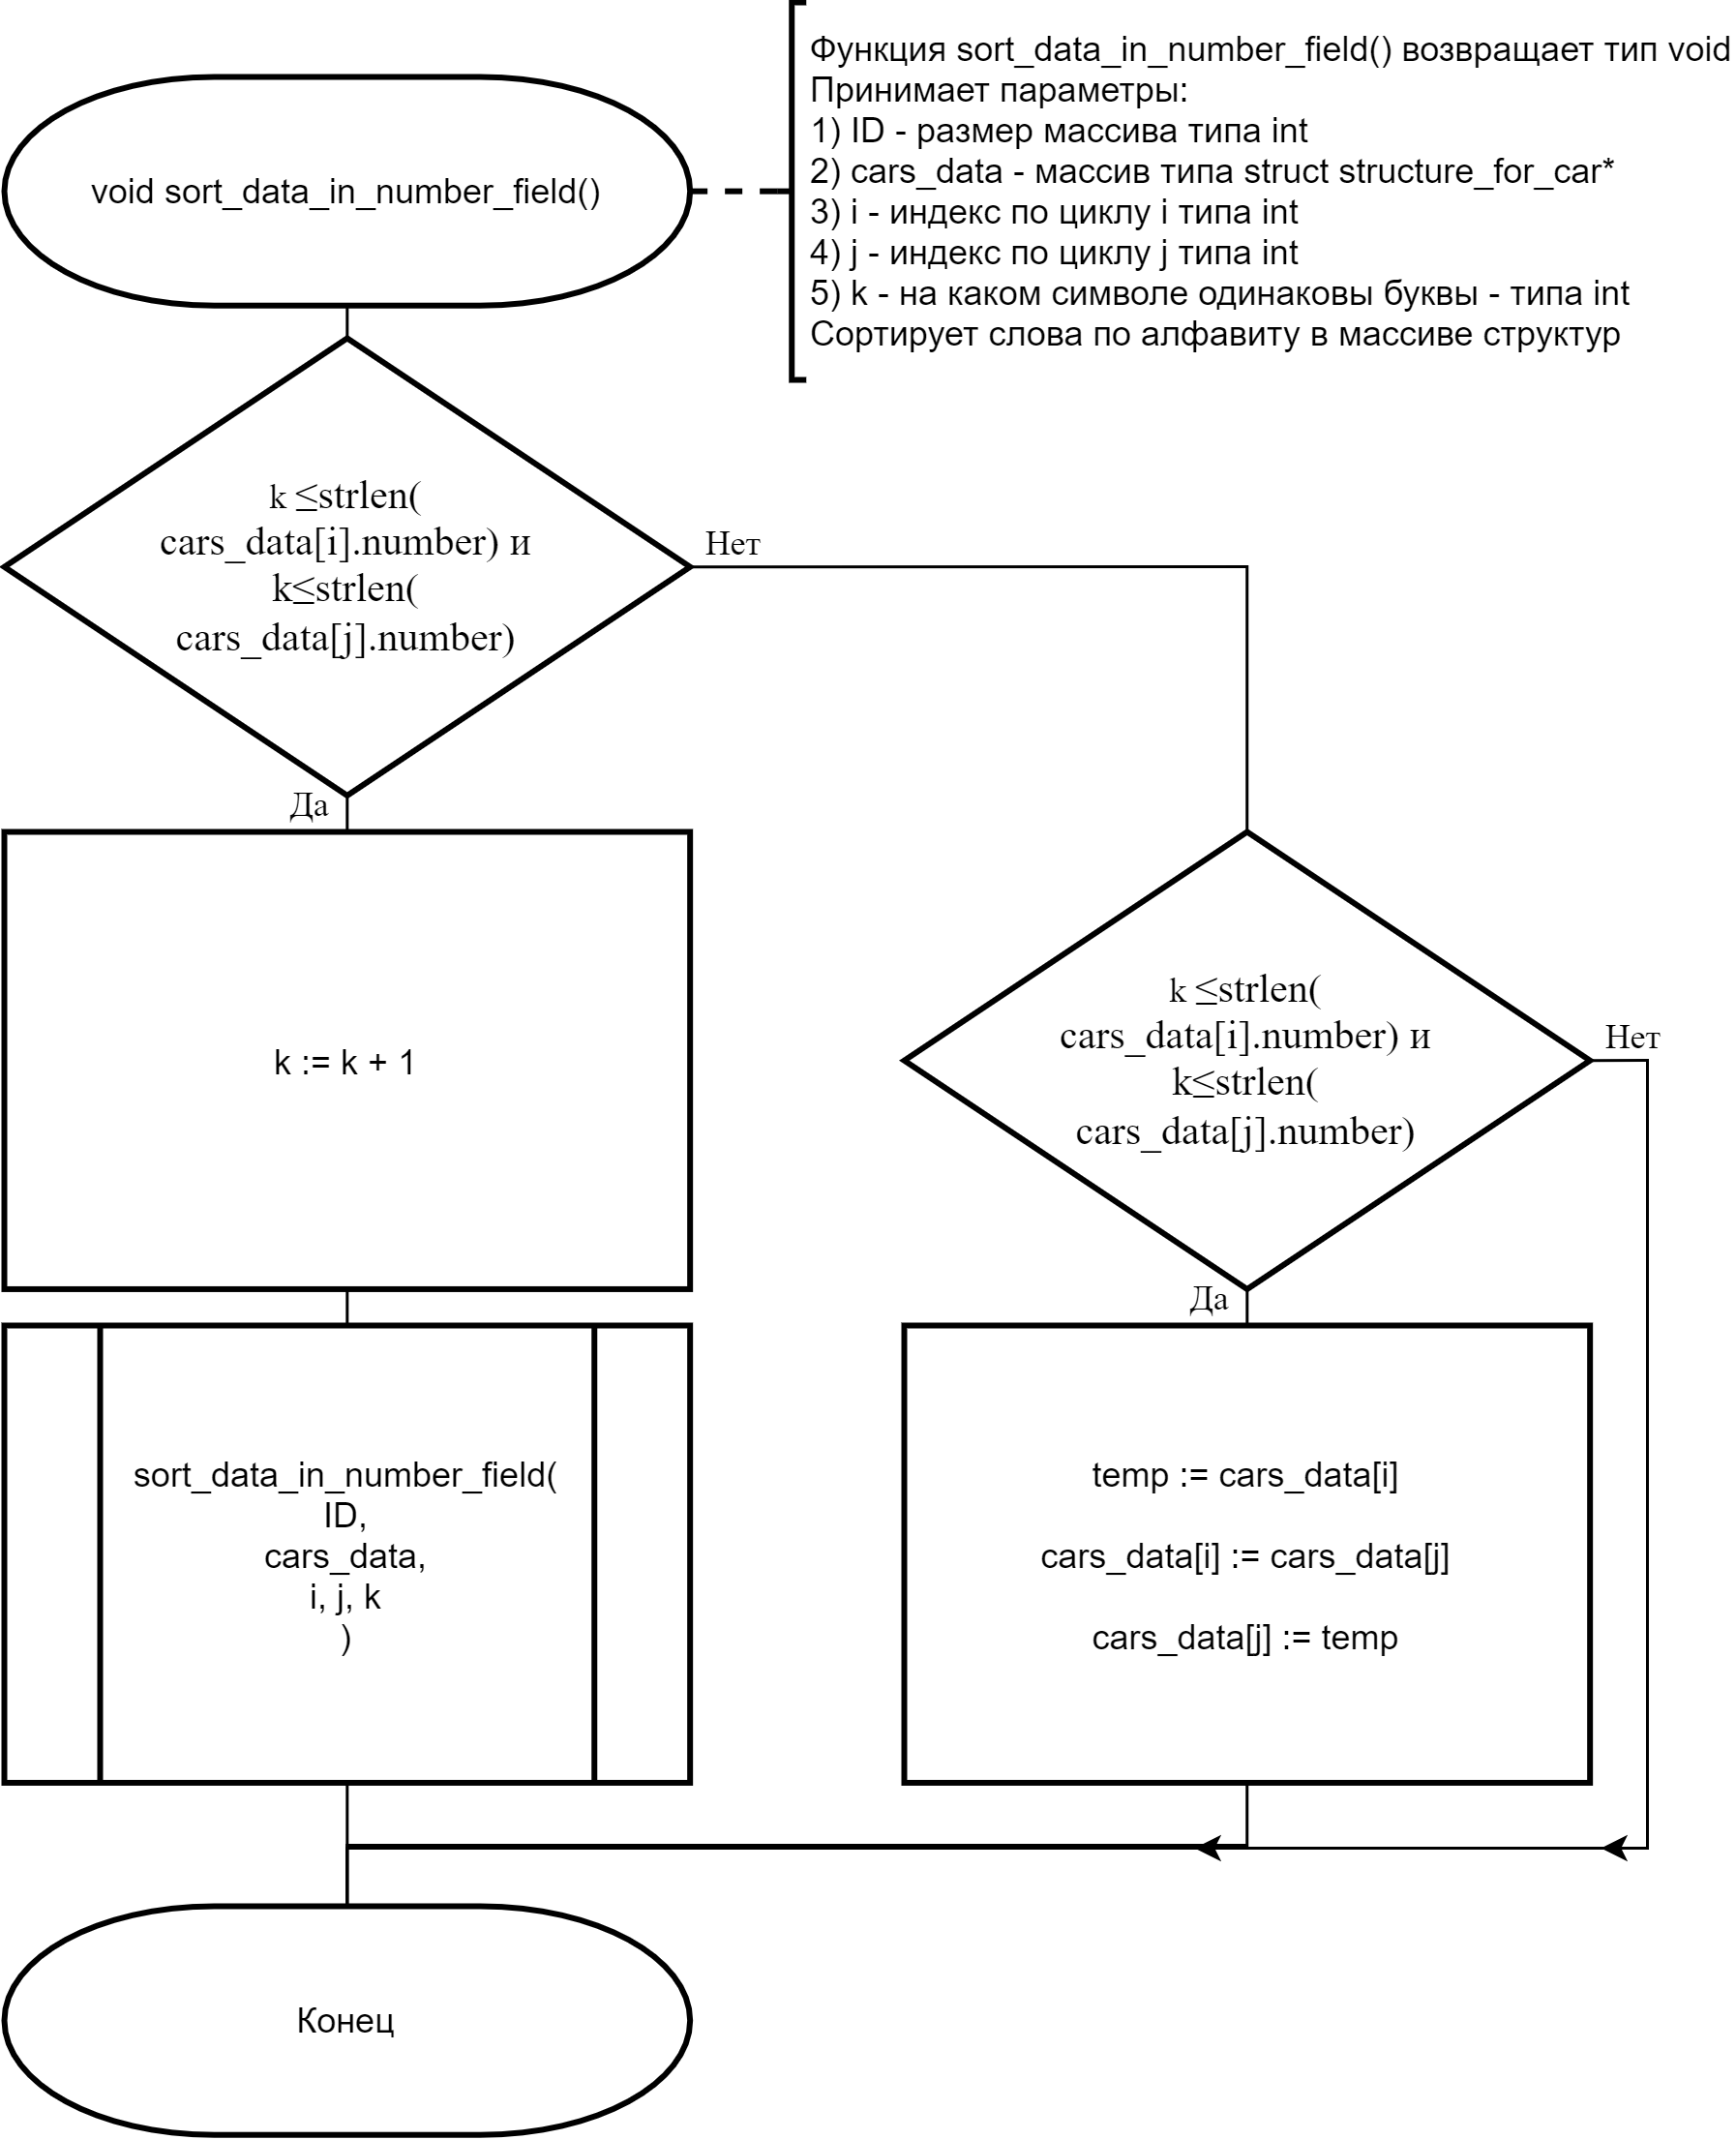
\includegraphics[]{../13/src/lab/menu/sort_data/get_sorted_array/sort_data_in_number_field/sort_data_in_number_field.png}
    }
    \caption{sort\_data\_in\_number\_field()}
    \label{fig:sort_data_in_number_field}
\end{figure}

\lstinputlisting[
	language=C,
	name=sort\_data\_in\_number\_field.h
]{../13/src/lab/menu/sort_data/get_sorted_array/sort_data_in_number_field/sort_data_in_number_field.h}

\lstinputlisting[
	language=C,
	name=sort\_data\_in\_number\_field.c
]{../13/src/lab/menu/sort_data/get_sorted_array/sort_data_in_number_field/sort_data_in_number_field.c}

\newpage

    % = = = = = Исполняемая программа
    \newpage
    \subsection{Исполняемая программа}
        %<<<===
\subsection{Сохранение файла как *.tsv}

\begin{tcolorbox}
\begin{verbatim}
Меню:
1. Открыть файл
2. Ввод данных       
3. Вывод данных      
4. Сортирова по полю 
5. Удалить запись    
6. Сохранить как     
0. Выйти из программы
\end{verbatim}
\end{tcolorbox}

Для вывода таблицы в консоль, выбираю из меню пункт 3.

\begin{tcolorbox}
\begin{verbatim}
| ID   | байт Номер    | байт Марка    | байт Фамилия      | Осмотр     |
| ---- | ---- -------- | ---- -------- | ---- ------------ | ---------- |
| 0    | 8    m74y7d   | 10   Alpha    | 10   Podushkin    | Не пройден |
| 1    | 8    d4rh75   | 4    Ford     | 10   Kamerov      | Не пройден |
| 2    | 8    fruf45   | 3    BMW      | 10   Rozetkov     | Пройден    |
Нажмите любую клавишу для продолжения...
\end{verbatim}
\end{tcolorbox}

Чтобы вернуться в меню нажимаю любую клавишу.

\begin{tcolorbox}
\begin{verbatim}
Меню:
1. Открыть файл
2. Ввод данных       
3. Вывод данных      
4. Сортирова по полю 
5. Удалить запись    
6. Сохранить как     
0. Выйти из программы
\end{verbatim}
\end{tcolorbox}

Попал в главное меню. Чтобы сохранить файл, выбираю пункт 6.

\begin{tcolorbox}
\begin{verbatim}
Меню:
1. Сохранить как tsv файл
2. Сохранить как bin файл
0. Выйти
\end{verbatim}
\end{tcolorbox}

Появилось меню. Так как нужно сохранить в *.tsv формате, то выбираю пункт 1. TSV - Tab Separated Values файл. Это файл как таблица. Открыть таблицу можно, например, в Libre Office Calc (Скриншот на рисунке \ref{fig:data-tsv}). Также можно такие файлы просматривать на GitHub (Скриншот на рисунке \ref{fig:data-tsv-on-github}).

\begin{figure}[p]
    \center{
        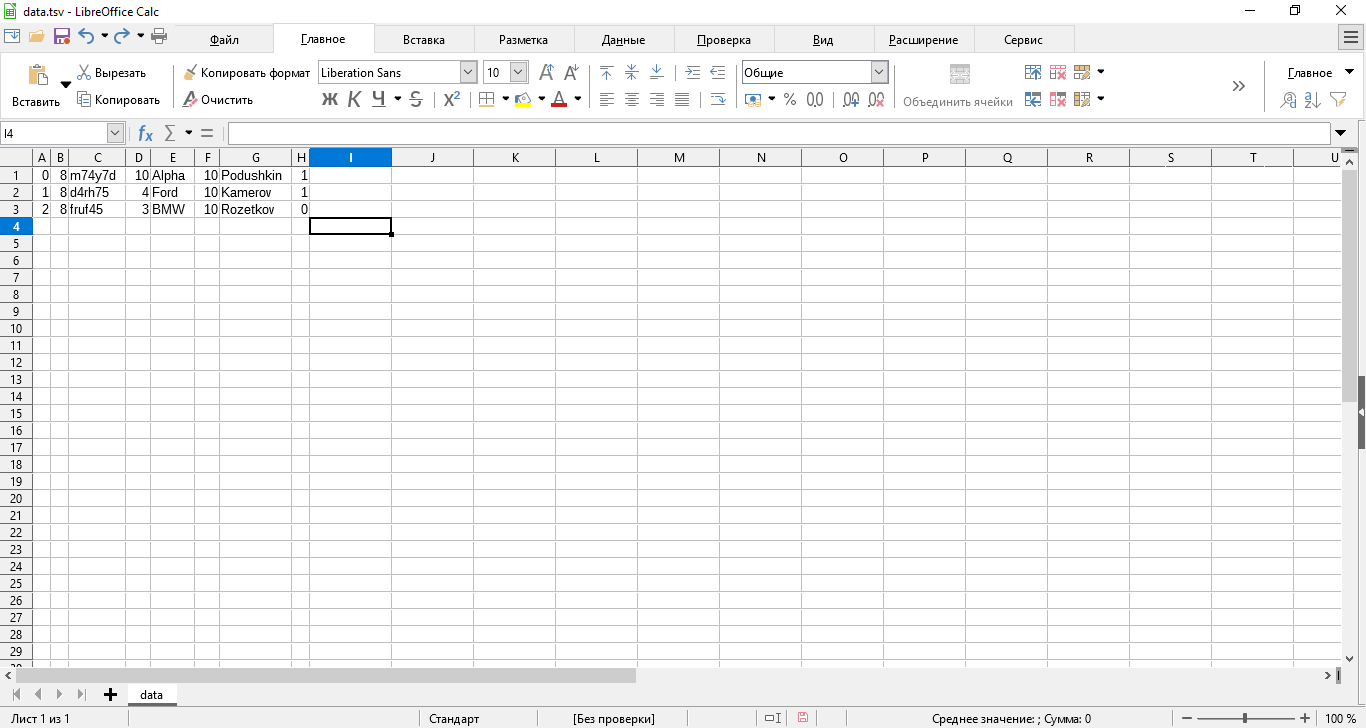
\includegraphics[width=16cm]{../pics/data-tsv-on-libre-office-calc.png}
    }
    \caption{data.tsv}
    \label{fig:data-tsv}
\end{figure}

\begin{figure}[p]
    \center{
        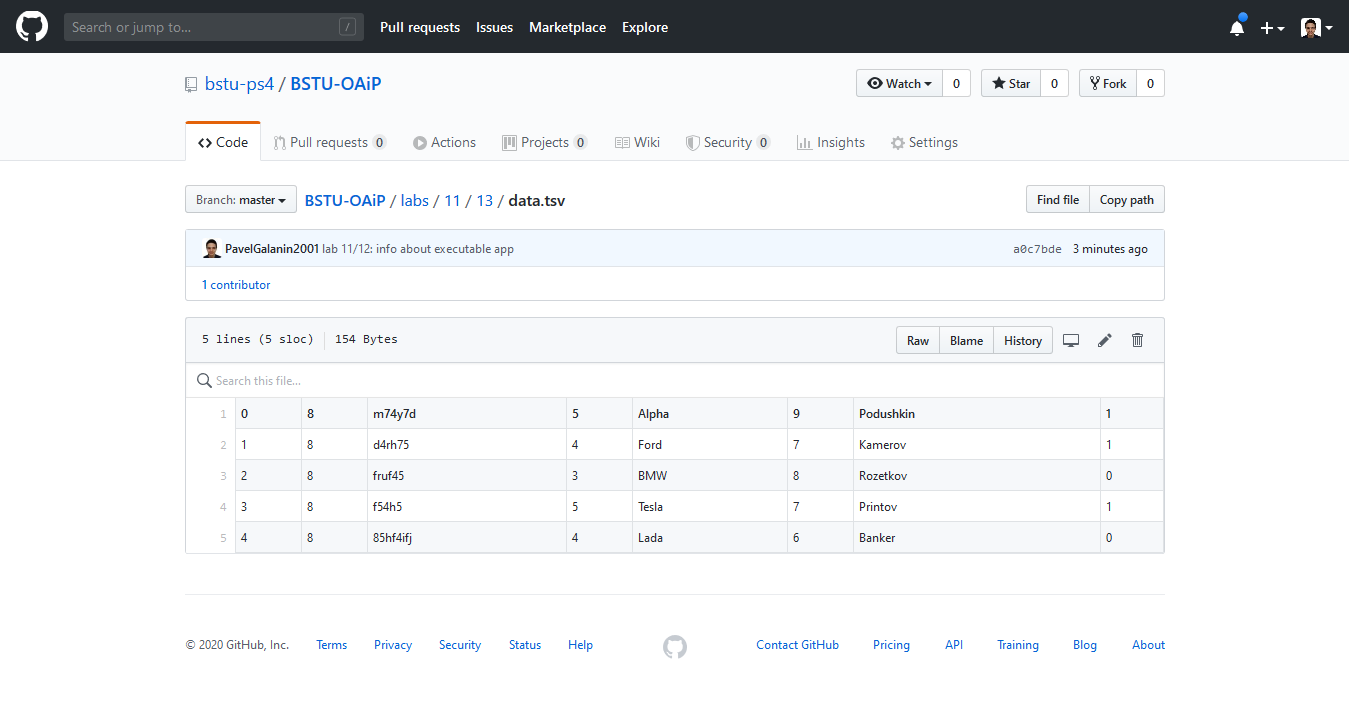
\includegraphics[width=16cm]{../pics/data-tsv-on-github.png}
    }
    \caption{data.tsv}
    \label{fig:data-tsv-on-github}
\end{figure}

Если открыть файл data.tsv, то там видем, что всё через табуляцию:
\begin{tcolorbox}
\begin{verbatim}
0	8	m74y7d	10	Alpha	10	Podushkin	1
1	8	d4rh75	4	Ford	10	Kamerov	1
2	8	fruf45	3	BMW	10	Rozetkov	0
\end{verbatim}
\end{tcolorbox}
%===>>>

\newpage

%<<<===
\subsection{Сохранение файла как *.bin}

\begin{tcolorbox}
\begin{verbatim}
Меню:
1. Открыть файл
2. Ввод данных
3. Вывод данных
4. Сортирова по полю
5. Удалить запись
6. Сохранить как
0. Выйти из программы
\end{verbatim}
\end{tcolorbox}

Для вывода таблицы в консоль, выбираю из меню пункт 3.
\begin{tcolorbox}
\begin{verbatim}
| ID   | байт Номер    | байт Марка    | байт Фамилия      | Осмотр     |
| ---- | ---- -------- | ---- -------- | ---- ------------ | ---------- |
| 0    | 8    m74y7d   | 5    Alpha    | 9    Podushkin    | Не пройден |
| 1    | 8    d4rh75   | 4    Ford     | 7    Kamerov      | Не пройден |
| 2    | 8    fruf45   | 3    BMW      | 8    Rozetkov     | Пройден    |
| 3    | 8    f54h5    | 5    Tesla    | 7    Printov      | Не пройден |
| 4    | 8    85hf4ifj | 4    Lada     | 6    Banker       | Пройден    |
Нажмите любую клавишу для продолжения...
\end{verbatim}
\end{tcolorbox}

Для выхода в меню, жму любую клавишу.

Попадаю в главное меню. Для сохранения файла, выбираю пункт 6.

\begin{tcolorbox}
\begin{verbatim}
Меню:
1. Сохранить как tsv файл
2. Сохранить как bin файл
0. Выйти
\end{verbatim}
\end{tcolorbox}

Появилось меню. Для сохранения в формате bin файла, выбираю пункт 2.

Появился файл data.bin (рисунок \ref{fig:far_folder}).

\begin{figure}[p]
    \center{
        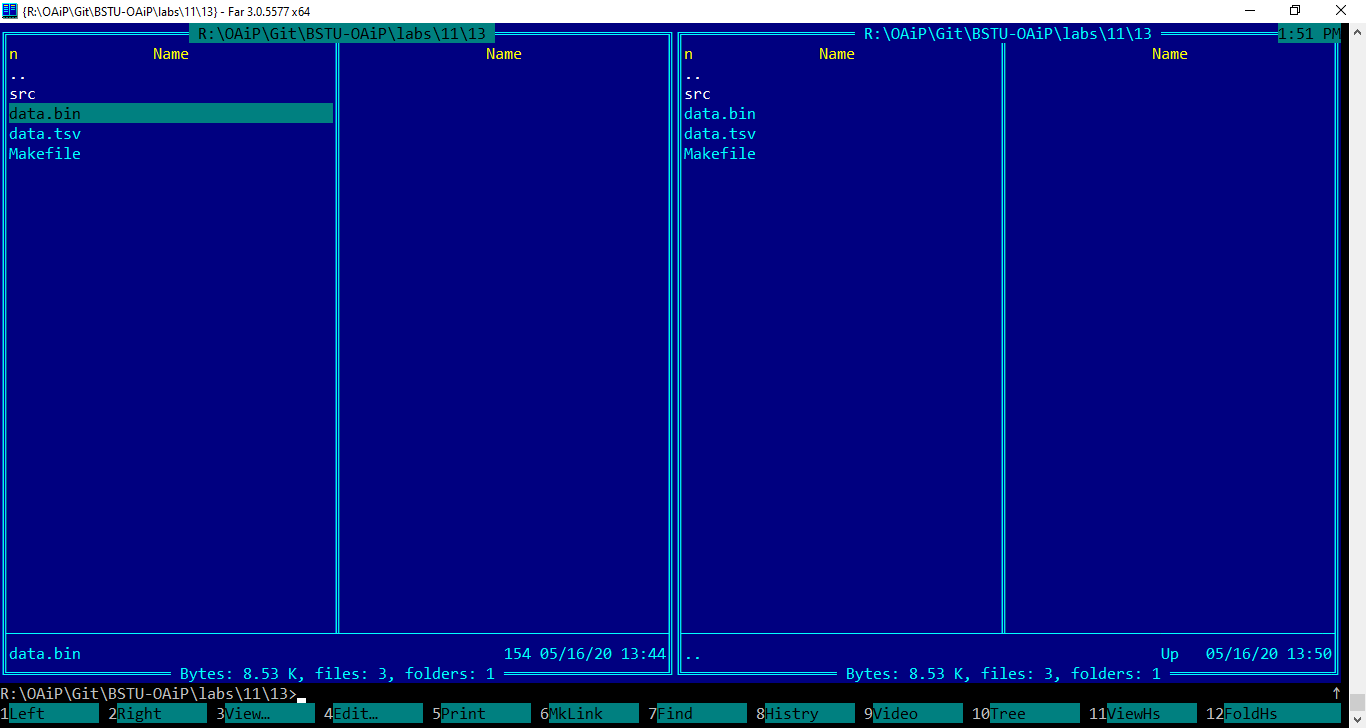
\includegraphics[width=16cm]{../pics/far-folder.png}
    }
    \caption{Бинарный файл в папке}
    \label{fig:far_folder}
\end{figure}

Открываю файл по нажатию F3. Видем как сохранился файл на рисунке \ref{fig:far_data_bin}.

\begin{figure}[p]
    \center{
        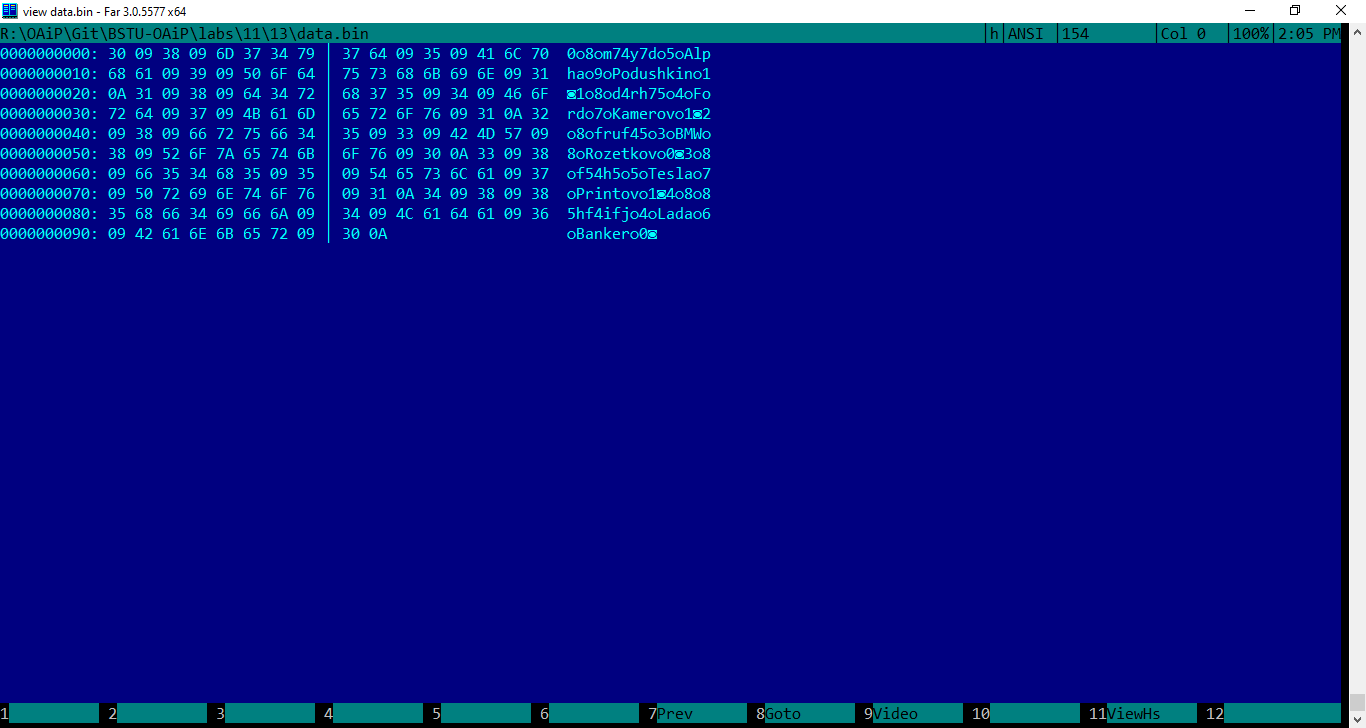
\includegraphics[width=16cm]{../pics/far-data-bin.png}
    }
    \caption{Бинарный файл в папке}
    \label{fig:far_data_bin}
\end{figure}
%===>>>

\newpage

%<<<===
\subsection{Открытие файла}

\begin{tcolorbox}
\begin{verbatim}
Меню:
1. Открыть файл      
2. Ввод данных       
3. Вывод данных      
4. Сортирова по полю 
5. Удалить запись    
6. Сохранить как     
0. Выйти из программы
\end{verbatim}
\end{tcolorbox}

Для вывода таблицы выбираю пункт 3.

\begin{tcolorbox}
\begin{verbatim}
| ID   | байт Номер    | байт Марка    | байт Фамилия      | Осмотр     |
| ---- | ---- -------- | ---- -------- | ---- ------------ | ---------- |
Нажмите любую клавишу для продолжения...
\end{verbatim}
\end{tcolorbox}

Видем, что таблица пустая. Для выхода в главное меню, жму любую клавишу.

У меня есть файл data.tsv. Он содержит такую информацию:
\begin{tcolorbox}
\begin{verbatim}
0	8	m74y7d	5	Alpha	9	Podushkin	1
1	8	d4rh75	4	Ford	7	Kamerov	1
2	8	fruf45	3	BMW	8	Rozetkov	0
3	8	f54h5	5	Tesla	7	Printov	1
4	8	85hf4ifj	4	Lada	6	Banker	0    
\end{verbatim}
\end{tcolorbox}

Захожу в свою программу. Из меню выбираю пункт 1, чтобы открыть файл.

\begin{tcolorbox}
\begin{verbatim}
Размер пути файла: 
\end{verbatim}
\end{tcolorbox}

Ввожу размер пути файла.

\begin{tcolorbox}
\begin{verbatim}
Размер пути файла: 10
Какой файл открыть:     
\end{verbatim}
\end{tcolorbox}

Ввожу путь до файла. У меня это \textbf{data.tsv}. Попадаю в главное меню. В меню выбираю пунтк 3, чтобы вывести таблицу в консоль.

\begin{tcolorbox}
\begin{verbatim}
| ID   | байт Номер    | байт Марка    | байт Фамилия      | Осмотр     |
| ---- | ---- -------- | ---- -------- | ---- ------------ | ---------- |
| 0    | 8    m74y7d   | 5    Alpha    | 9    Podushkin    | Не пройден |
| 1    | 8    d4rh75   | 4    Ford     | 7    Kamerov      | Не пройден |
| 2    | 8    fruf45   | 3    BMW      | 8    Rozetkov     | Пройден    |
| 3    | 8    f54h5    | 5    Tesla    | 7    Printov      | Не пройден |
| 4    | 8    85hf4ifj | 4    Lada     | 6    Banker       | Пройден    |
Нажмите любую клавишу для продолжения...   
\end{verbatim}
\end{tcolorbox}

\begin{tcolorbox}
\begin{verbatim}
Меню:
1. Открыть файл      
2. Ввод данных       
3. Вывод данных      
4. Сортирова по полю 
5. Удалить запись    
6. Сохранить как     
0. Выйти из программы
\end{verbatim}
\end{tcolorbox}

Для открытия файла, выбираю 1 пункт в меню.

\begin{tcolorbox}
\begin{verbatim}
Размер пути файла: 
\end{verbatim}
\end{tcolorbox}

Ввожу размер пути файла. (Это для создания динамической строки)

\begin{tcolorbox}
\begin{verbatim}
Размер пути файла: 8
Какой файл открыть: 
\end{verbatim}
\end{tcolorbox}

\begin{tcolorbox}
\begin{verbatim}
Меню:
1. Открыть файл      
2. Ввод данных       
3. Вывод данных      
4. Сортирова по полю 
5. Удалить запись    
6. Сохранить как     
0. Выйти из программы
\end{verbatim}
\end{tcolorbox}

В меню выбираем пункт 3 для вывода таблицы.

\begin{tcolorbox}
\begin{verbatim}
| ID   | байт Номер    | байт Марка    | байт Фамилия      | Осмотр     |
| ---- | ---- -------- | ---- -------- | ---- ------------ | ---------- |
| 0    | 8    m74y7d   | 5    Alpha    | 9    Podushkin    | Не пройден |
| 1    | 8    d4rh75   | 4    Ford     | 7    Kamerov      | Не пройден |
| 2    | 8    fruf45   | 3    BMW      | 8    Rozetkov     | Пройден    |
| 3    | 8    f54h5    | 5    Tesla    | 7    Printov      | Не пройден |
| 4    | 8    85hf4ifj | 4    Lada     | 6    Banker       | Пройден    |
Нажмите любую клавишу для продолжения...
\end{verbatim}
\end{tcolorbox}
%===>>>

\newpage

%<<<===
\subsection{Если файл не найден}

\begin{tcolorbox}
\begin{verbatim}
Меню:
1. Открыть файл      
2. Ввод данных       
3. Вывод данных      
4. Сортирова по полю 
5. Удалить запись    
6. Сохранить как     
0. Выйти из программы
\end{verbatim}
\end{tcolorbox}

Выбираю из меню пункт 1, чтобы открыть файл. Ввожу размер файла и не существующий путь

\begin{tcolorbox}
\begin{verbatim}
Размер пути файла: 
\end{verbatim}
\end{tcolorbox}

Ввожу размер пути файла. (Это для создания динамической строки)
    
\begin{tcolorbox}
\begin{verbatim}
Размер пути файла: 8
Какой файл открыть: uirg
\end{verbatim}
\end{tcolorbox}

Ввожу не существующий путь.

\begin{tcolorbox}
\begin{verbatim}
Файл не найден!

Меню:
1. Открыть файл
0. Выйти в главное меню
\end{verbatim}
\end{tcolorbox}

Появилось сообщение, что файл не найден. Появилось меню, чтобы выйти в главное меню, и чтобы остаться открывать файл.
%===>>>

    % = = = = = Вывод ЛР
    \labconclusion{}

% = = = = =
\newpage
\section{Бинарные и текстовые файлы}
    % = = = = = Условие
    \subsection{Условие}
        В программу разработанную в лабораторной работе 10 добавить чтение и сохранение данных массива структур при помощи бинарных файлов следующим образом:
\begin{itemize}
    \item При первом запуске программы должен создаваться бинарный или текстовый файл на выбор пользователя для хранения данных из массива структур.
    \item При добавлении новой записи в массив структур в файл должна дописываться новая запись, без изменения остальных записей.
    \item При повторном запуске программы, если файл уже существует, то информация в массив структур должна читаться из этого файла. Если файл отсутствует, то он должен создаваться (см. Пункт 1).
    \item Все изменения (сортировка, изменения полей записи, удаление записи) – сохраняются в файле при помощи полной перезаписи содержимого.
    \item Сделать вывод о том, какие преимущества использования конкретного типа файлов (бинарные или текстовые) в решаемой вами задаче.
\end{itemize}


    % = = = = = Исходный код
    \newpage
    \subsection{Исходный код}
        \subsubsection{open\_file()}

%Блок-схема на рисунке \ref{fig:open\_file}.

%\begin{figure}[p]
%    \center{
%        \includegraphics[]{../13/src/lab/menu/open_file/open_file.png}
%    }
%    \caption{open\_file()}
%    \label{fig:open_file}
%\end{figure}

\lstinputlisting[
    language=C,
    name=open\_file.h
]{../13/src/lab/menu/open_file/open_file.h}

\lstinputlisting[
    language=C,
    name=open\_file.c
]{../13/src/lab/menu/open_file/open_file.c}

\newpage
\subsection{save\_as()}

Блок-схема на рисунке \ref{fig:save_as}.

\begin{figure}[p]
    \center{
        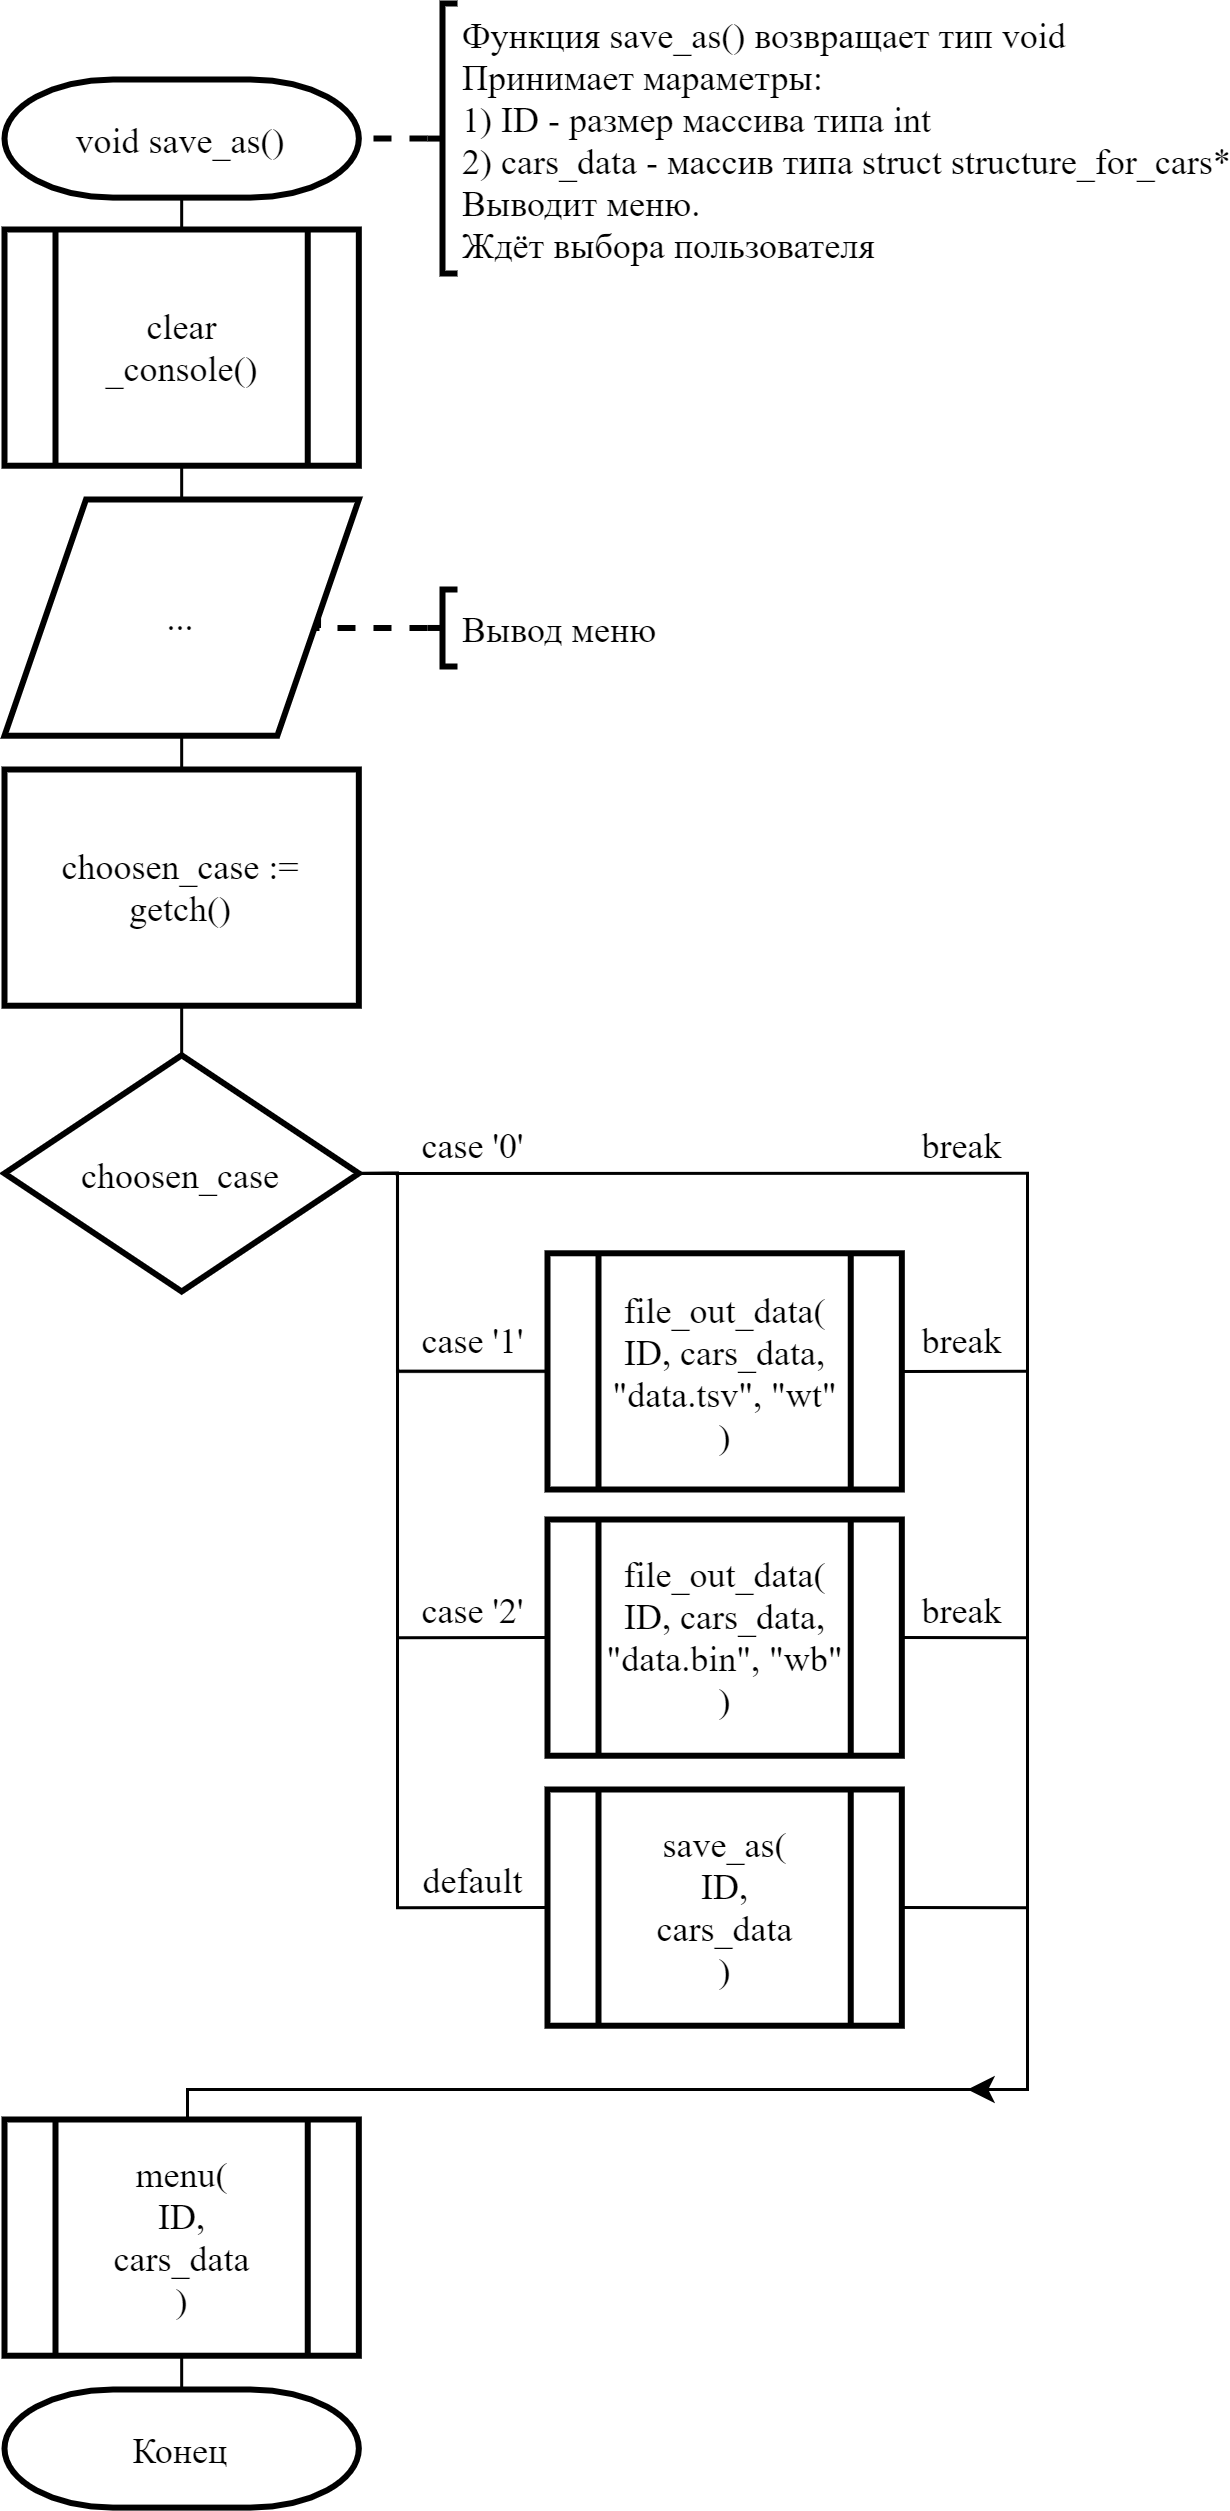
\includegraphics[]{../13/src/lab/menu/save_as/save_as.png}
    }
    \caption{save\_as()}
    \label{fig:save_as}
\end{figure}

\lstinputlisting[
    language=C,
    name=save_as.h
]{../13/src/lab/menu/save_as/save_as.h}

\lstinputlisting[
    language=C,
    name=save_as.c
]{../13/src/lab/menu/save_as/save_as.c}

\newpage
\subsubsection{file\_out\_data()}

%Блок-схема на рисунке \ref{fig:file_out_data}.

%\begin{figure}[p]
%    \center{
%        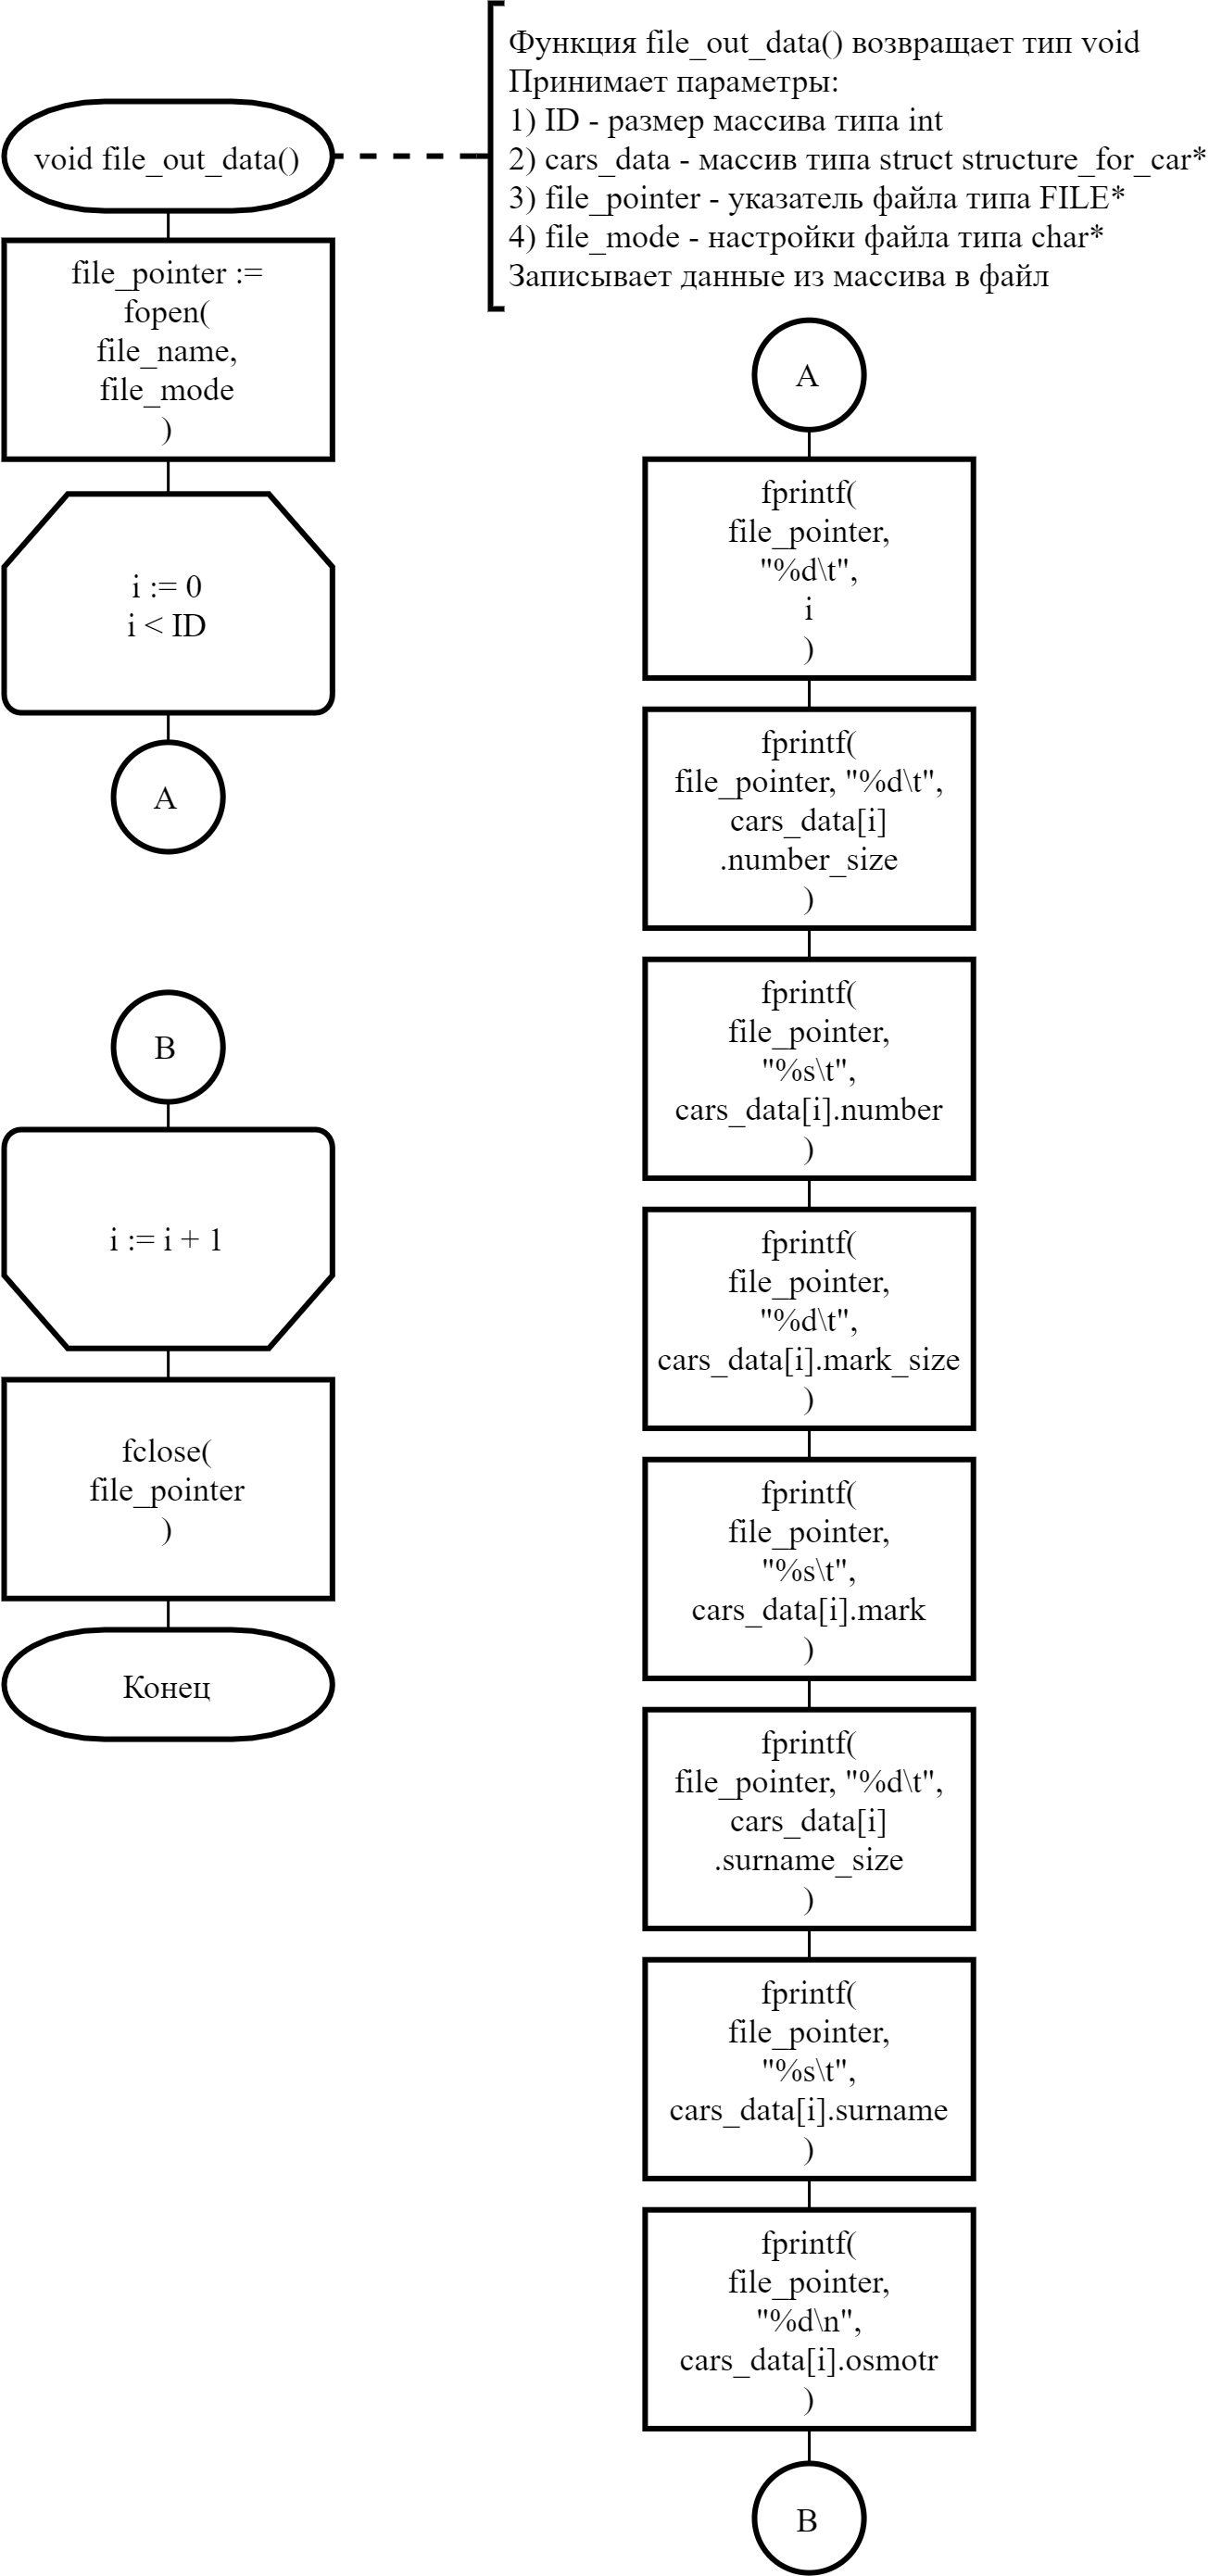
\includegraphics[]{../13/src/lab/menu/save_as/file_out_data/file_out_data.png}
%    }
%    \caption{file\_out\_data()}
%    \label{fig:file_out_data}
%\end{figure}

\lstinputlisting[
    language=C,
    name=file\_out\_data.h
]{../13/src/lab/menu/save_as/file_out_data/file_out_data.h}

\lstinputlisting[
    language=C,
    name=file\_out\_data.c
]{../13/src/lab/menu/save_as/file_out_data/file_out_data.c}

\newpage


    % = = = = = Исполняемая программа
    \newpage
    \subsection{Исполняемая программа}
        % = = = = = Сохранение файла как *.tsv

\subsubsection{Сохранение файла как *.tsv}

Из меню выбираю бункт 3, для вывода таблицы в консоль.

\begin{tcolorbox}
\begin{verbatim}
| ID   | байт Номер    | байт Марка    | байт Фамилия      | Осмотр     |
| ---- | ---- -------- | ---- -------- | ---- ------------ | ---------- |
| 0    | 8    m74y7d   | 10   Alpha    | 10   Podushkin    | Не пройден |
| 1    | 8    d4rh75   | 4    Ford     | 10   Kamerov      | Не пройден |
| 2    | 8    fruf45   | 3    BMW      | 10   Rozetkov     | Пройден    |
Нажмите любую клавишу для продолжения...
\end{verbatim}
\end{tcolorbox}

Нажимаю любую клавишу. Выбираю из меню пункт 6, чтобы сохранить файл.

\begin{tcolorbox}
\begin{verbatim}
Меню:
1. Сохранить как tsv файл
2. Сохранить как bin файл
0. Выйти
\end{verbatim}
\end{tcolorbox}

Выбираю пункт 1, чтобы сохранить как tsv файл. TSV - Tab Separated Values файл. Открыть таблицу можно, например, в Libre Office Calc (Скриншот на рисунке \ref{fig:data-tsv}). Также можно такие файлы просматривать на GitHub (Скриншот на рисунке \ref{fig:data-tsv-on-github}).

Если открыть файл, то там:
\begin{tcolorbox}
\begin{verbatim}
0	8	m74y7d	10	Alpha	10	Podushkin	1
1	8	d4rh75	4	Ford	10	Kamerov	1
2	8	fruf45	3	BMW	10	Rozetkov	0
\end{verbatim}
\end{tcolorbox}

\begin{figure}[h]
    \center{
        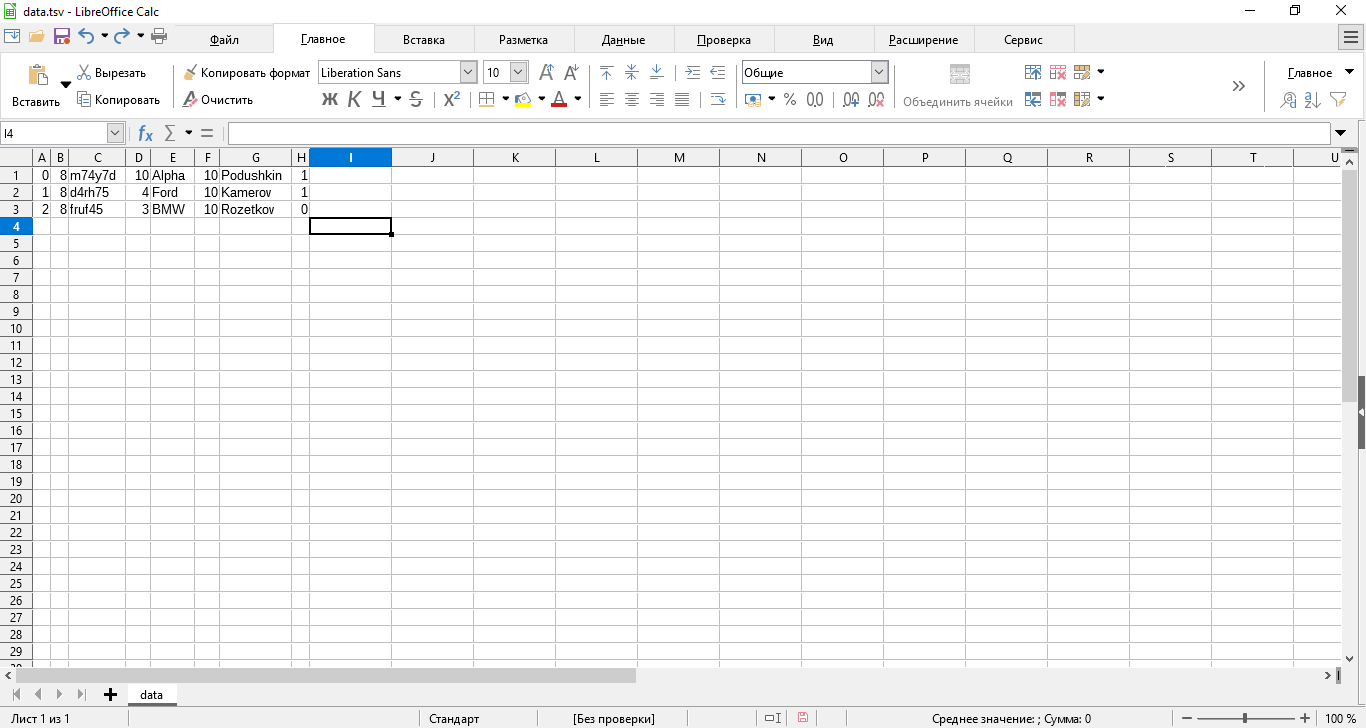
\includegraphics[width=16cm]{../pics/data-tsv-on-libre-office-calc.png}
    }
    \caption{data.tsv}
    \label{fig:data-tsv}
\end{figure}

\begin{figure}[h]
    \center{
        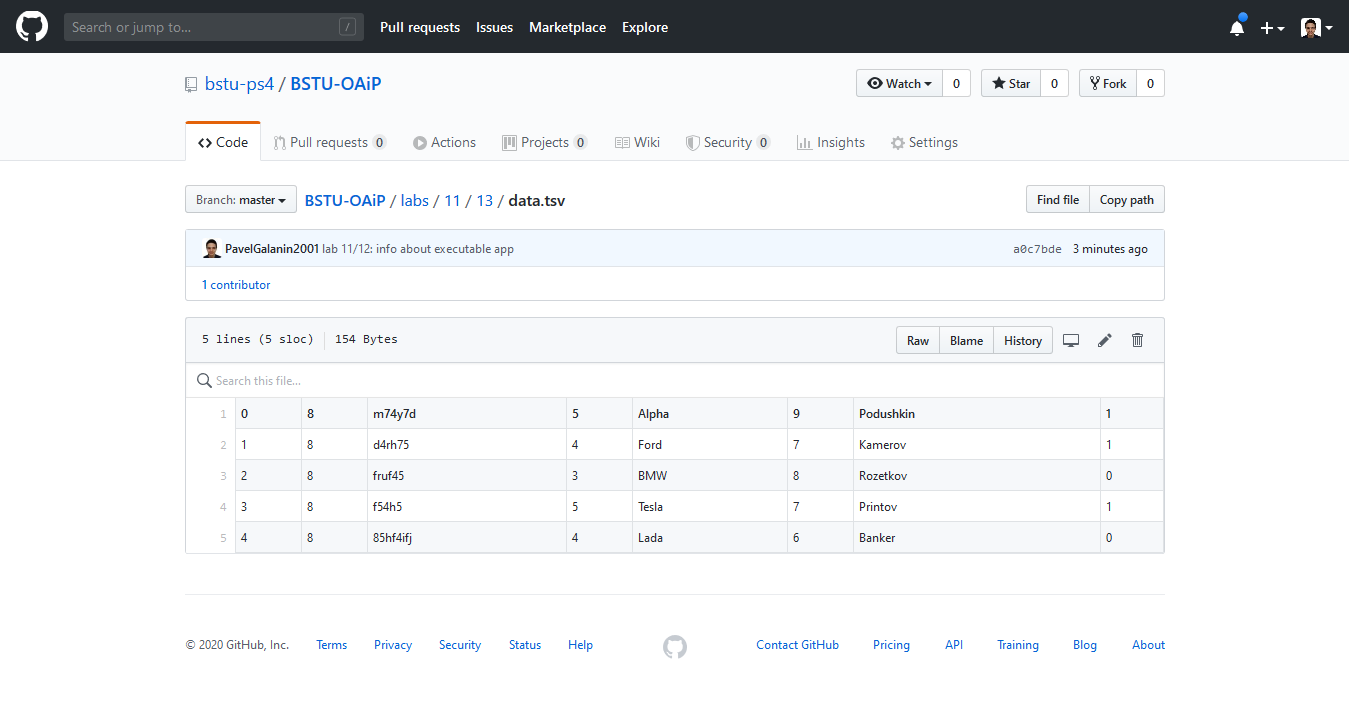
\includegraphics[width=16cm]{../pics/data-tsv-on-github.png}
    }
    \caption{data.tsv}
    \label{fig:data-tsv-on-github}
\end{figure}

% = = = = = Открытие файла

\subsubsection{Открытие файла}

Проредактировав поля в Libre Office Calc, файл содержит:

\begin{tcolorbox}
\begin{verbatim}
0	8	m74y7d	5	Alpha	9	Podushkin	1
1	8	d4rh75	4	Ford	7	Kamerov	1
2	8	fruf45	3	BMW	8	Rozetkov	0
3	8	f54h5	5	Tesla	7	Printov	1
4	8	85hf4ifj	4	Lada	6	Banker	0
\end{verbatim}
\end{tcolorbox}

Захожу в свою программу. Из меню выбираю пункт 1, чтобы открыть файл.

\begin{tcolorbox}
\begin{verbatim}
Размер пути файла: 
\end{verbatim}
\end{tcolorbox}

Ввожу размер пути файла.

\begin{tcolorbox}
\begin{verbatim}
Размер пути файла: 10
Какой файл открыть:     
\end{verbatim}
\end{tcolorbox}

Ввожу путь до файла. У меня это \textbf{data.tsv}. В консоли всякая информация, что файл сохранен в струтуру.

\begin{verbatim}
Размер пути файла: 10
Какой файл открыть: data.tsv
 = = = = = case 0 = = = = =
0
 = = = = = case 1 = = = = =
8
 = = = = = case 2 = = = = =
m74y7d
 = = = = = case 3 = = = = =
5
 = = = = = case 4 = = = = =
Alpha
 = = = = = case 5 = = = = =
9
 = = = = = case 6 = = = = =
Podushkin
 = = = = = case 7 = = = = =
1
 = = = = = case 0 = = = = =
1
 = = = = = case 1 = = = = =
8
 = = = = = case 2 = = = = =
d4rh75
 = = = = = case 3 = = = = =
4
 = = = = = case 4 = = = = =
Ford
 = = = = = case 5 = = = = =
7
 = = = = = case 6 = = = = =
Kamerov
 = = = = = case 7 = = = = =
1
 = = = = = case 0 = = = = =
2
 = = = = = case 1 = = = = =
8
 = = = = = case 2 = = = = =
fruf45
 = = = = = case 3 = = = = =
3
 = = = = = case 4 = = = = =
BMW
 = = = = = case 5 = = = = =
8
 = = = = = case 6 = = = = =
Rozetkov
 = = = = = case 7 = = = = =
0
 = = = = = case 0 = = = = =
3
 = = = = = case 1 = = = = =
8
 = = = = = case 2 = = = = =
f54h5
 = = = = = case 3 = = = = =
5
 = = = = = case 4 = = = = =
Tesla
 = = = = = case 5 = = = = =
7
 = = = = = case 6 = = = = =
Printov
 = = = = = case 7 = = = = =
1
 = = = = = case 0 = = = = =
4
 = = = = = case 1 = = = = =
8
 = = = = = case 2 = = = = =
85hf4ifj
 = = = = = case 3 = = = = =
4
 = = = = = case 4 = = = = =
Lada
 = = = = = case 5 = = = = =
6
 = = = = = case 6 = = = = =
Banker
 = = = = = case 7 = = = = =
0
Нажмите любую клавишу для продолжения...
\end{verbatim}

Нажимаю любую клавишу. В меню выбираю пунтк 3, чтобы вывести таблицу в консоль.

\begin{tcolorbox}
\begin{verbatim}
| ID   | байт Номер    | байт Марка    | байт Фамилия      | Осмотр     |
| ---- | ---- -------- | ---- -------- | ---- ------------ | ---------- |
| 0    | 8    m74y7d   | 5    Alpha    | 9    Podushkin    | Не пройден |
| 1    | 8    d4rh75   | 4    Ford     | 7    Kamerov      | Не пройден |
| 2    | 8    fruf45   | 3    BMW      | 8    Rozetkov     | Пройден    |
| 3    | 8    f54h5    | 5    Tesla    | 7    Printov      | Не пройден |
| 4    | 8    85hf4ifj | 4    Lada     | 6    Banker       | Пройден    |
Нажмите любую клавишу для продолжения...   
\end{verbatim}
\end{tcolorbox}

Структуры успешно обновилась.

\subsection{Если файл не найден}

Выбираю из меню пункт 1, чтобы открыть файл. Ввожу размер файла и не существующий путь

\begin{tcolorbox}
\begin{verbatim}
Размер пути файла: 10
Какой файл открыть: uirg
\end{verbatim}
\end{tcolorbox}

Появиться сообщение, что файл не найден. Также будет меню, чтобы выйти в главное меню, либо же остаться открывать файл.

\begin{tcolorbox}
\begin{verbatim}
Файл не найден!

Меню:
1. Открыть файл
0. Выйти в главное меню
\end{verbatim}
\end{tcolorbox}


    % = = = = = Вывод ЛР
    \labconclusion{}

% = = = = = Литература
\newpage
\begin{thebibliography}{3}
    \bibitem{}
    БрГТУ.ПОИТ. Лабораторная работа "Структуры, перечисления, объединения"
    \bibitem{}
    БрГТУ.ПОИТ. Лабораторная работа "Бинарные и текстовые файлы"
\end{thebibliography}

\textbf{Ссылки}
\begin{itemize}
    \item Репозиторий с исходным кодом\\
    https://github.com/bstu-ps4/BSTU-OAiP
\end{itemize}

\end{document}